\chapter[Air entrainment by impingement of liquid jet on a pool]{Air entrainment by jet impingement\footnote{The results presented in this chapter are published in: Sanjay, V and Das, A. K. (2017). \textquotedblleft On air entrainment in a water pool by impingement of a jet\textquotedblright. AIChE Journal, 63.11, pp. 5169 -- 5181. DOI : \href{https://onlinelibrary.wiley.com/doi/abs/10.1002/aic.15828}{\color{black}10.1002/aic.15828}.}}\label{Chapter::BubbleEntrainment}
\section{Introduction}
In this chapter, the investigation of air entrainment due to impingement of a water jet on a pool is studied extensively to understand the physics of the initiation and the cluster of bubbles formed below the free surface. A look around reveals the presence of this phenomenon in everyday life, ranging from filling of a glass of water using tap to several chemical reactions, such as mineral flotation, steel teeming process and gas absorption. \citet{Evans1996} defines a plunging liquid jet as a moving column of liquid that passes through a gaseous head-space before impinging on the horizontal free surface. In his review work, \citet{Bin1993} reviewed previous works in the area of the impinging jet in a pool and showed the application of the same in the field of wastewater treatment. Entrainment is desirable in processes like aeration reactions during wastewater treatment whereas it is undesirable in processes such as pouring of molten metals during casting or glass molding. Hence, it is important to understand the physics behind this phenomenon so that the processes it affects, directly or indirectly, can be optimized. Possible outcomes due to the jet impingement in a pool have been identified as smooth free surface without entrainment or formation of rigorous bubble cluster below the jet-pool contact \citep{Roy2013}. A triangular entrained region is found to be a three-dimensional association of disconnected bubble population continuously breaking and making with the neighbors \citep{Belden2012,Harby2014,Bagatur2014}. A correlation for prediction of maximum entrained height for a range of jet diameters and lengths is proposed. The trajectory of a single bubble is also studied to understand the kinematics of the bubble cluster. Alongside, an electrical conductivity probe has been used to examine the probabilistic presence of the bubble at a given depth in the liquid pool. 
\section{Experimental setup and methodology}
An in-house experimental setup to investigate the phenomenon of air entrainment by impinging liquid jet is developed. Figure~\ref{Fig::setup} (a) illustrates the schematic of this experimental facility. A water pool in a Plexiglas tank (0.5 $m$ x 0.5 $m$ x 0.5 $m$), is impinged by a water jet (with properties as given in Table~\ref{Table::liqProperties}). The flow of the jet is controlled using valves and is measured with a calibrated rota-meter at ambient conditions. Arrangements are made to lower the jet for variation of its height from the pool ($l_j$). Further, the jet diameter ($d_j$) can be changed by using different guiding nozzles. The injection system is kept as sufficiently long $(\sim 120D)$ to obtain fully developed velocity profile in the injected water jet. \\
Noticing the dynamics of the problem, it is realized that the depth of the entrainment ($d_s$) is dependent on the kinematic or geometric control parameters, such as the diameter of the jet ($d_j$), velocity of the jet ($u_j$), its length ($l_j$) along with other physical variables such as the density of the liquid ($\rho_l$), viscosity ($\mu_l$), surface tension, $\sigma$ and acceleration due to gravity ($g$). 
\begin{equation}
d_s = \Phi(u_j, d_j, \rho_l, \mu_l, \sigma, g) 
\label{Equation::params}
\end{equation}
\begin{figure}
	\centering
	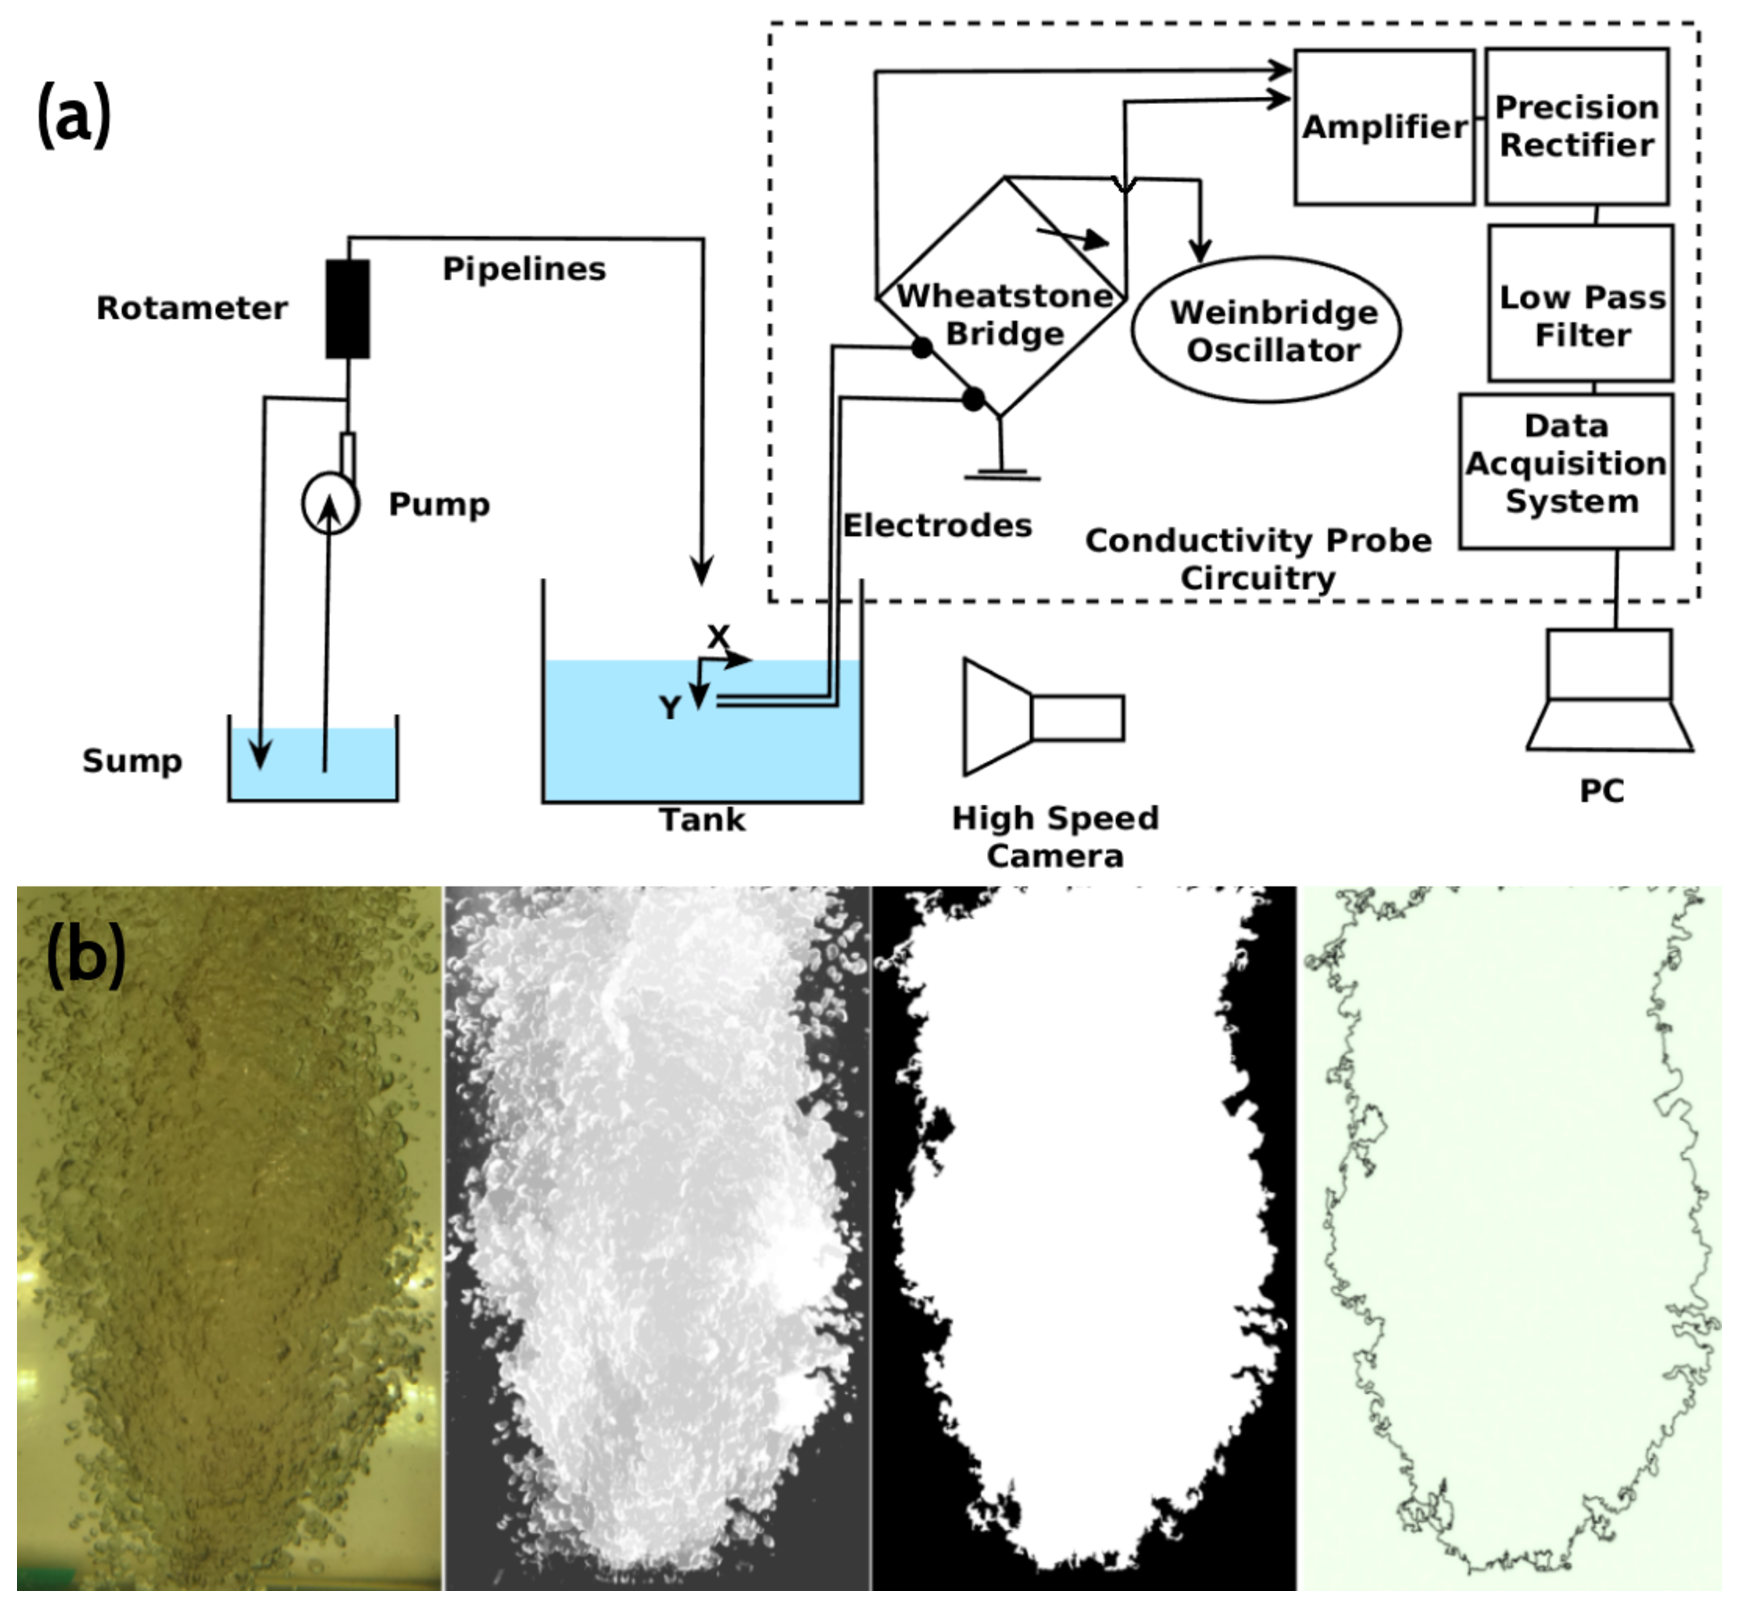
\includegraphics[width = 0.95\linewidth]{chapters/jetPool/Figure1}
	\caption{(a) In house developed experimental setup for the study of entrainment process. The coordinate system has been defined using the Cartesian system centered at the point of impact of the jet on the pool. (b) Sequence of image processing applied for the characterization of the bubble cluster.}
	\label{Fig::setup}
\end{figure}
Assuming, $u_j$, $d_j$ and $\rho_l$ as the repeating variables in equation~\ref{Equation::params}, the functional relation shown in equation~\ref{Equation::DimensionlessNumbers} is obtained. 
\begin{equation}\label{Equation::DimensionlessNumbers}
\frac{d_s}{d_j} = \Psi\left(\frac{\sqrt{gd_j}}{u_j}, \frac{l_j}{d_j}, \frac{\mu_l}{\rho_lu_jd_j}, \frac{\sigma}{\rho_lu_j^2d_j} \right)
\end{equation} 
\begin{table}
	\centering
	\caption{Details of the physical properties of the tap water used in the experiments and the ambient air conditions.}
	\begin{tabular}{@{}cccc@{}}
		\toprule
		Fluid & \begin{tabular}[c]{@{}c@{}}Density\\ ($kg/m^3$)\end{tabular} & \begin{tabular}[c]{@{}c@{}}Viscosity \\ ($Pas$)\end{tabular} & \begin{tabular}[c]{@{}c@{}}Surface Tension\\ ($Nm$)\end{tabular} \\ \midrule
		Water & 1000 & 0.001 & \multirow{2}{*}{0.072} \\
		Air & 1.24 & 1.8e-5 &  \\ \bottomrule
	\end{tabular}
	\label{Table::liqProperties}
\end{table}
\begin{table}
	\centering
	\caption{Variation of different parameters associated with the flow. The Reynolds number and the product of Froude numbers are based on jet characteristics}
	\begin{tabular}{@{}cccc@{}}
		\toprule
		\begin{tabular}[c]{@{}c@{}}Flow\\  Rate\\ (x $ 10 ^{-5} \: m^3/s$)\end{tabular} & \begin{tabular}[c]{@{}c@{}}Nozzle \\ Diameter\\ ($m$)\end{tabular} & \begin{tabular}[c]{@{}c@{}}Reynold's \\ Number \\ $Re$\end{tabular} & \begin{tabular}[c]{@{}c@{}}Froude \\ Numbers\\ $Fr_DFr_L$\end{tabular} \\ 
		\midrule
		$1.67$ to $100$  & 0.01 to 0.0256 & 2000 to 50000 & 1 to 4 \\
		\bottomrule
	\end{tabular}
	\label{Table::parameter}
\end{table}
The first term (inverse of the diametrical Froude number, $Fr_D$) is a measure of the inertia of the circular jet whereas the second term is directly associated with the gravitational potential available to the jet as it starts its descent towards the pool. Further, the last two terms can be identified as the inverse of the Reynolds and the Weber number. The diametrical Froude Number ($Fr_D$) and the jet length ratio ($\frac{l_j}{d_j}$) present the control aspects of these experiments and simulation. These terms can be combined into the product of the Froude Numbers and the uniqueness of a particular flow configuration is considered using the number, $Fr_DFr_L = \left[\frac{V}{\sqrt{gD_j}}\right]\left[\frac{V}{\sqrt{gl_j}}\right]$, where $Fr_L$ is the longitudinal Froude Number. Table~\ref{Table::parameter} contains the range of variations involved in the present study. The high-speed camera is used to capture the dynamic behavior of the entrainment process with a maximum frame rate of 2000 frames per second at full resolution. 
The raw images obtained from the high-speed camera are passed through RGB to grayscale conversion, noise removal by subtracting background and grayscale to black and white conversion stages. From temporal black and white images, feature extraction, like the centre of mass evaluation and area determination of cluster, are performed. Sobel technique is used for interface tracking using which is the maximum depth of entrainment penetration is determined. Figure~\ref{Fig::setup} (b) illustrates different stages of image analysis. \\
\begin{figure}
	\centering
	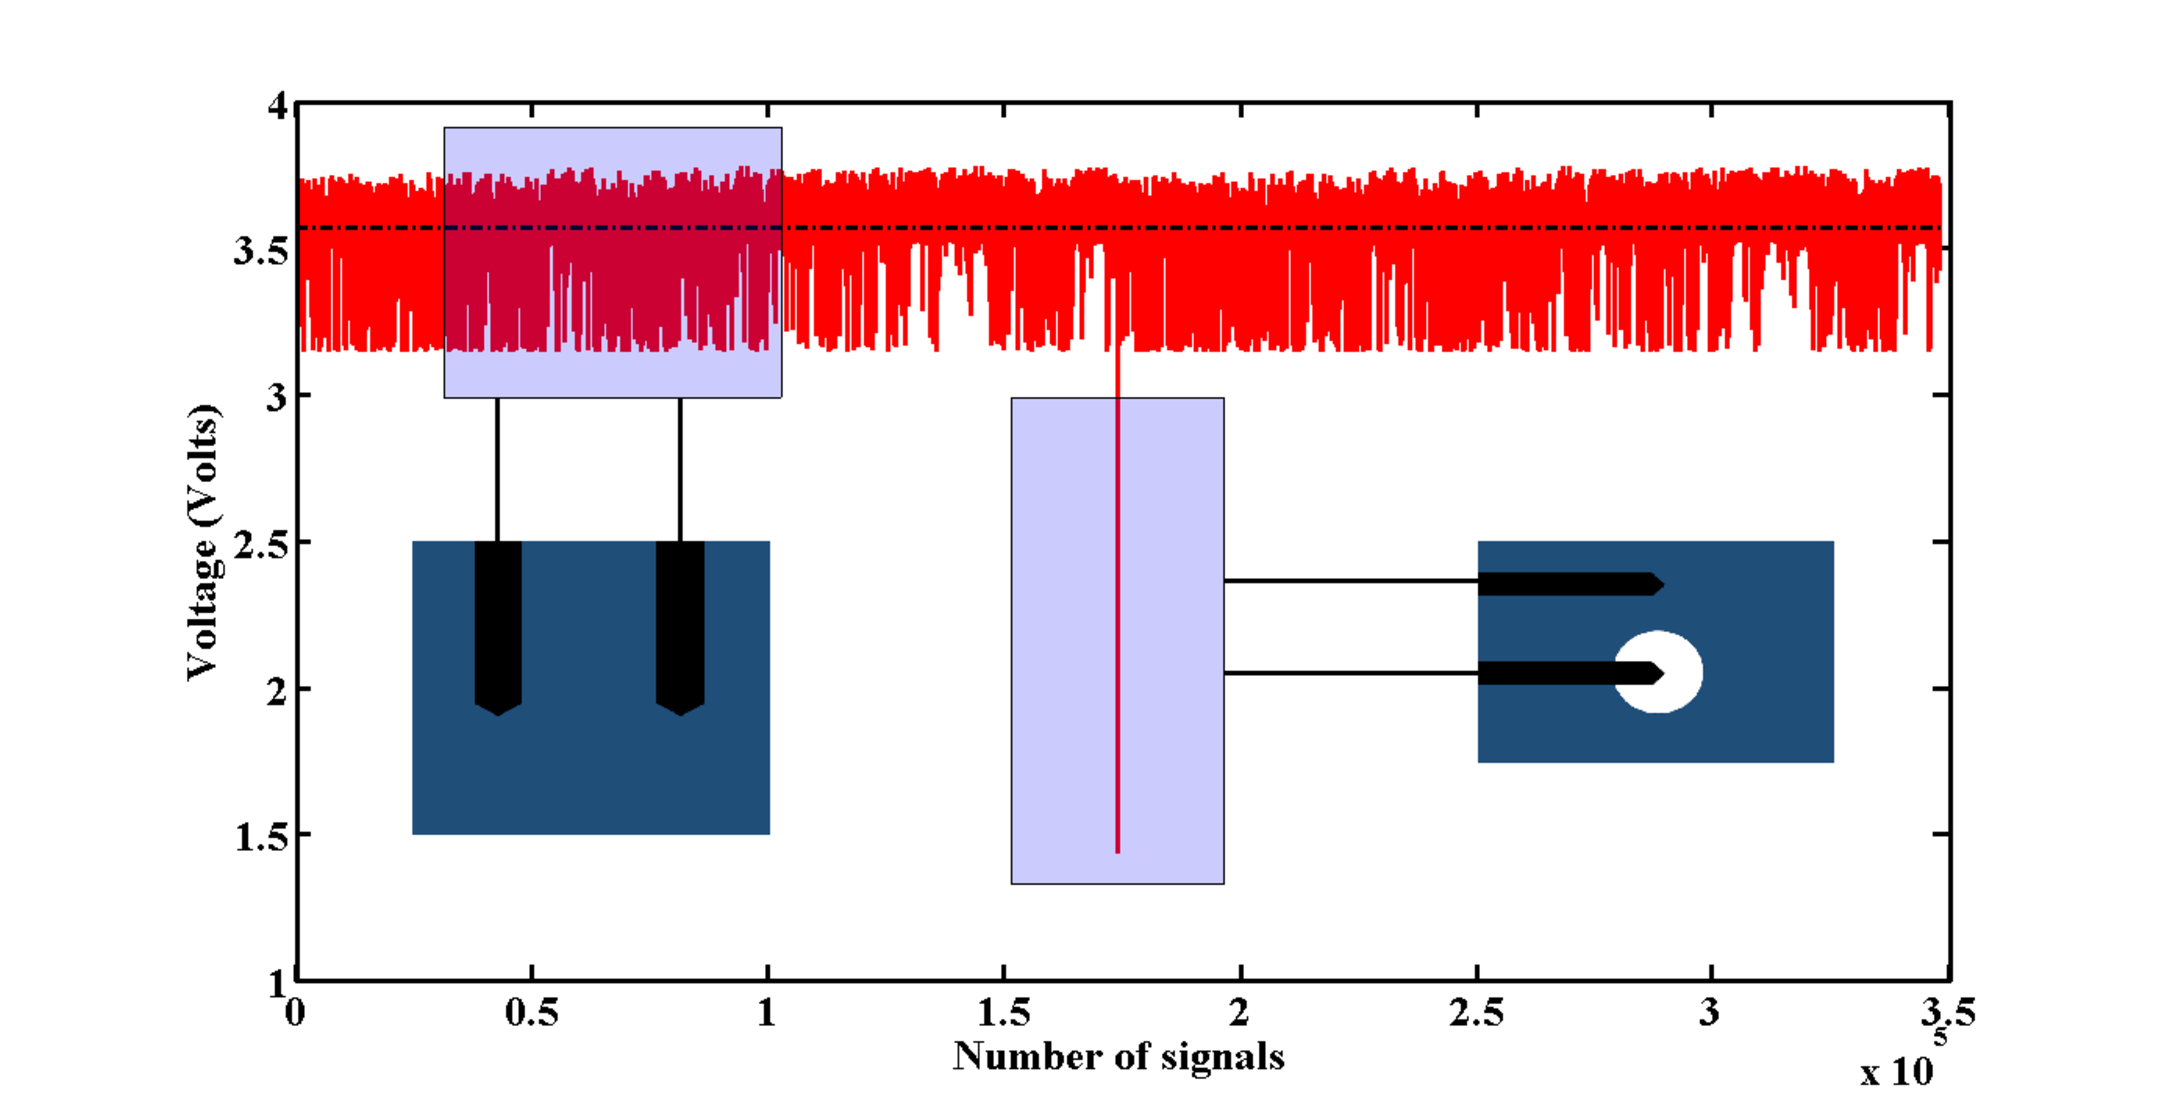
\includegraphics[width=\linewidth]{chapters/jetPool/Figure2}
	\caption{Signal behavior for different closure of circuitry. In case water closes the circuit the voltage signal is normal. However, with the presence of bubbles, an instantaneous dip can be observed}
	\label{Figure::show}
\end{figure}
Moreover, an electrical conductivity probe is developed to detect the presence of entrapped air bubbles at a given spatial coordinate in the liquid pool. The working principle of conductivity probe is variable resistance when different (air/water) medium closes the circuitry between two copper electrodes as illustrated in figure~\ref{Fig::setup} (a). To convert the instantaneous variable resistance into a measurable voltage signal, electronic circuitry has also been developed. Figure~\ref{Figure::show} gives an idea about the behavior of probe signals for different media completing the circuitry in between the electrodes. In the next section, the mathematical setup used for spatio-temporal fully resolved simulation of the process is explained. Care has been taken to accommodate at least 10 cells inside disconnected interface for accurate capture of the interfacial dynamics. No turbulence model is used in the model framework.
\section{Numerical model}
Bubble entrainment is studied in a three-dimensional finite volume framework using the Volume Of Fluid (VOF) approach for interface tracking. Open source solver, Gerris is used for the study \citep{Popinet2003}. It implements the finite volume discretization on an octree adaptive grid with piecewise linear VOF model. 
\begin{figure}
	\centering
	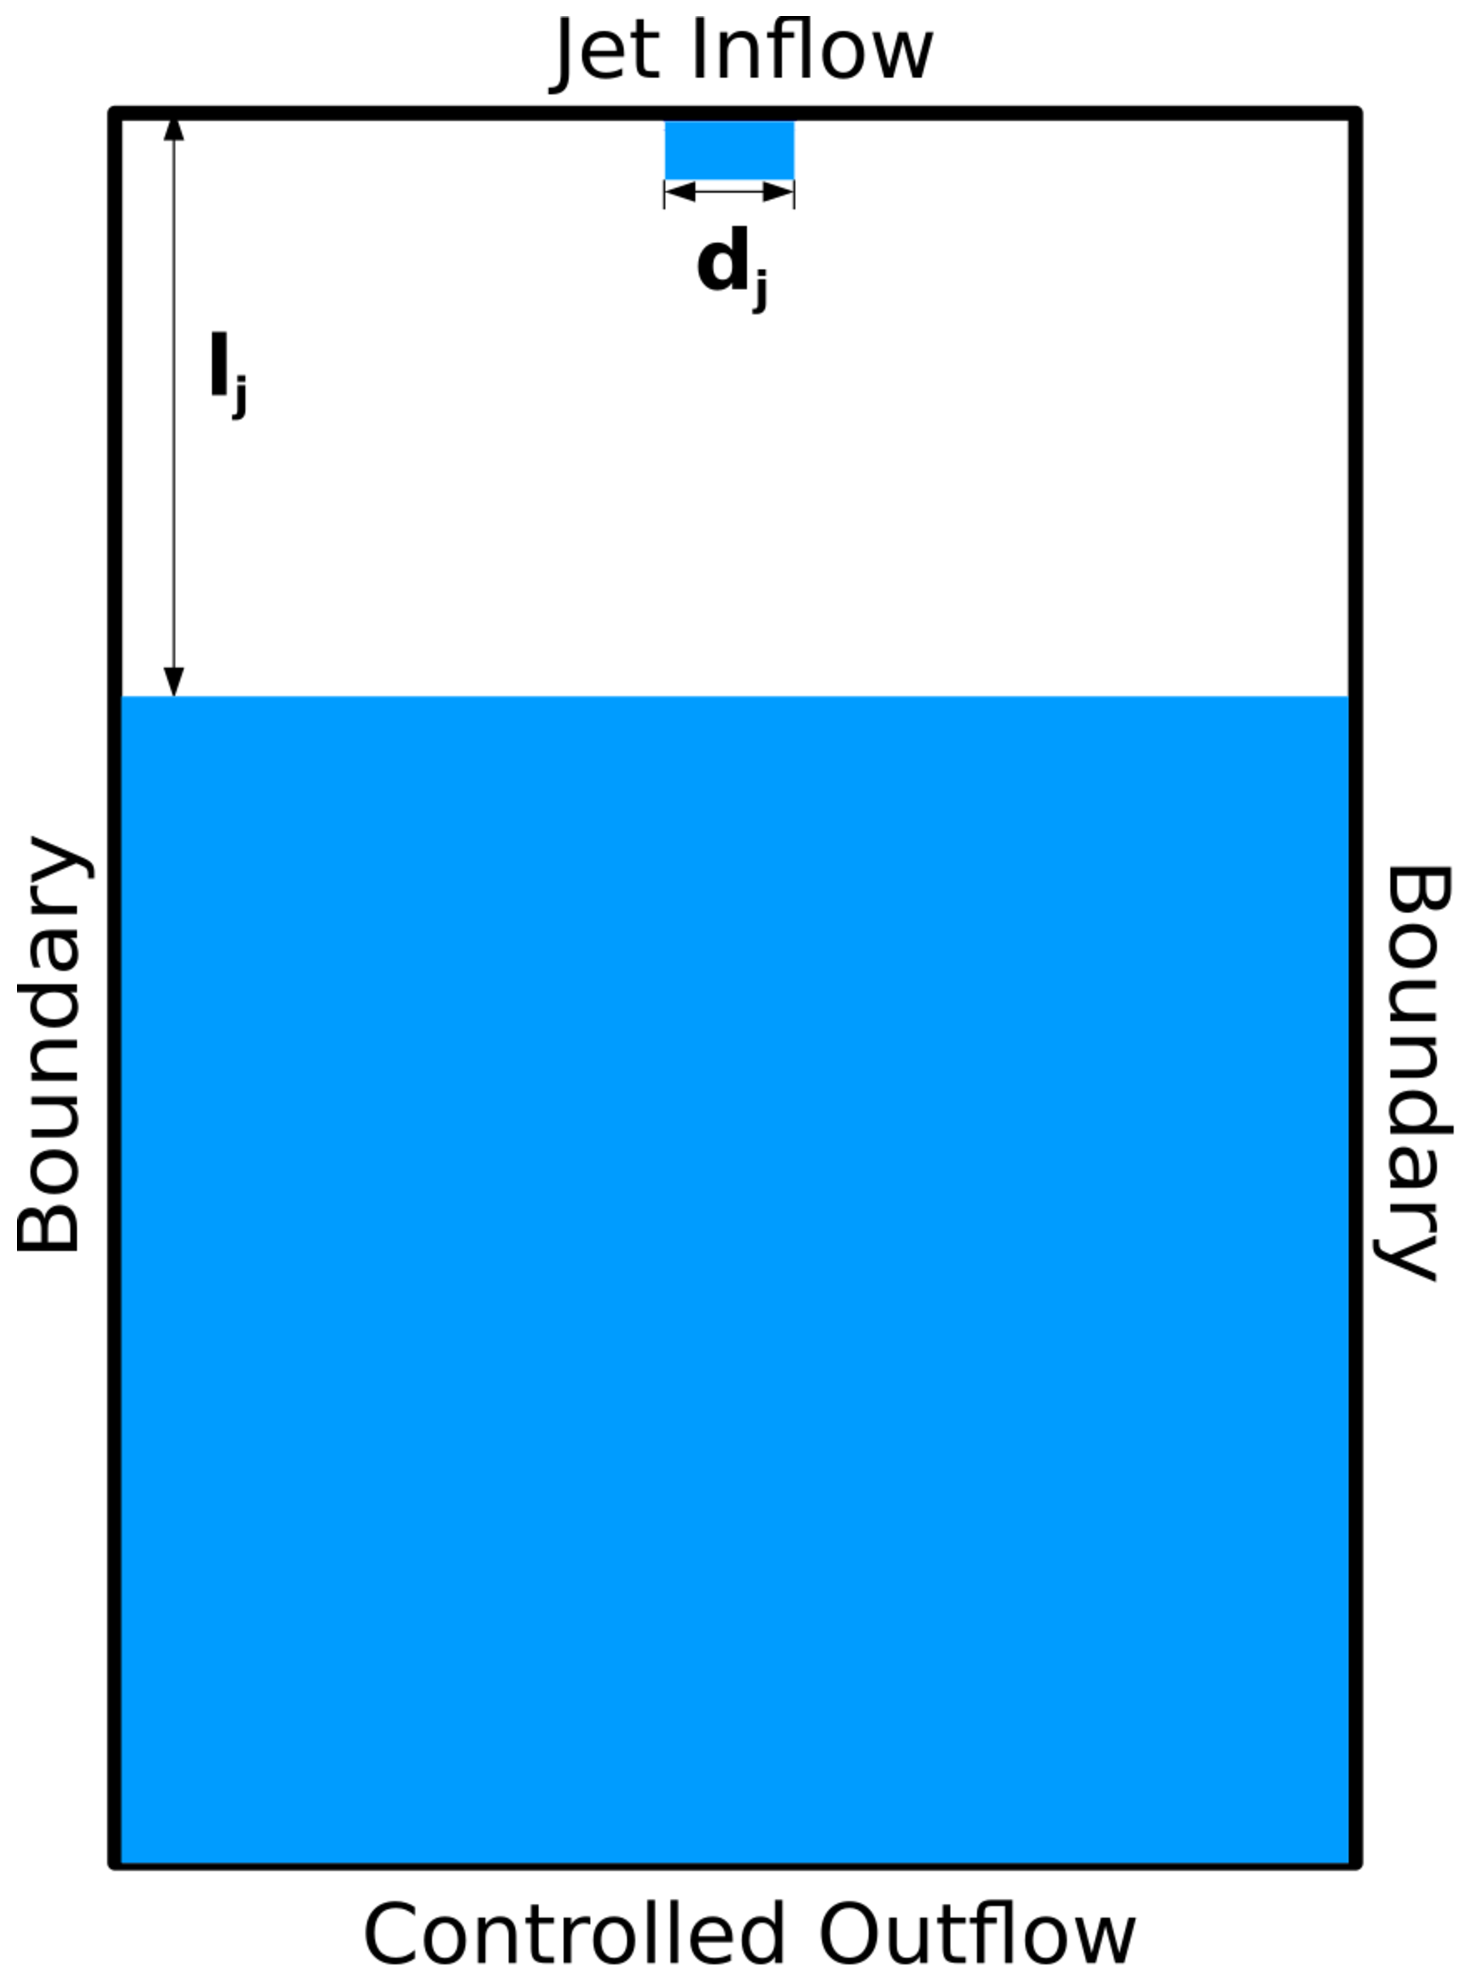
\includegraphics[width=0.5\linewidth]{chapters/jetPool/Figure3}
	\caption{The computational domain with the implemented boundary conditions.}
	\label{Figure::domain}
\end{figure}
\subsection{Setup of the numerical model}
Figure~\ref{Figure::domain} illustrates the computational domain with dimensions 30$d_j$ x 10$d_j$ x 10$d_j$. The lateral surfaces are modeled as boundaries using no-slip condition. The distance of these walls from the centerline of the jet ($5d_j$) is kept large to avoid any biasing from boundaries. The bottom boundary is given a controlled velocity out-flux condition, to ensure that the water level does not change whereas the top boundary has jet inflow and outflow boundary condition. A small jet is initialized at the start of the simulation, along with the water pool. The product of the Froude numbers ($Fr_DFr_L$) determines the average inlet velocity of the liquid jet and the velocity profile depends on the turbulent character of the jet. If the Reynolds number of the jet is below 2300 (laminar jet), parabolic profile $\left[2\left(1 - \left(\frac{2r}{d_j}\right)^2\right) \right]u_j$ is patched whereas power law velocity profile $\left[\frac{8}{7}\left(1 - \frac{2r}{d_j}\right)^{\frac{1}{7}} \right]u_j$ is used for turbulent jets. With the above mathematical model in place, mesh sensitivity analysis is carried out.\\
\begin{table}
	\centering
	\def~{\hphantom{0}}
	\begin{tabular}{ccccc}
		\toprule
		Case  &\begin{tabular}[c]{@{}c@{}} $\: \: \: \: \: \: \: \: \: \left(\frac{d_j}{\delta l}\right)_{max}$ \end{tabular}& \begin{tabular}[c]{@{}c@{}}Maximum \\ level \end{tabular} & \begin{tabular}[c]{@{}c@{}} $\: \: \: \: \: \: \: \: \: \left(\frac{d_j}{\delta l}\right)_{min}$ \end{tabular}& \begin{tabular}[c]{@{}c@{}}Minimum \\ level \end{tabular}\\[3pt]
		\midrule
		~1.  & ~6.4& ~6 & ~1.6&4\\
		~2.   & ~12.8& ~7 & ~1.6&4\\
		~3.  &  ~25.6& ~8 & ~1.6&4\\
		~4.   &  ~51.2& ~9 &  ~1.6&4\\
		~5. &  102.4&10& ~1.6&4\\
		~6. & 204.8&11 & ~1.6&4\\
		~7. & 102.4&10 & ~3.2&5\\
		~8. & 102.4&10&~6.4&6\\
		~9. & 102.4&10&~12.8&7\\
		10. & 102.4&10 &~25.6&8\\
		\bottomrule
	\end{tabular}
	\caption{Designation of cases considered for the grid sensitivity analysis.}
	\label{Table::CaseGis}
\end{table}
Refinement is bestowed adaptively based on the gradient of the volume fraction of fluid $\alpha(x_i,t)$. This ensures that the number of cells around the interface is sufficient enough to capture small-scale variations. Let, $\delta l$ be the size of a cell, which is non-dimensionalized as $\frac{d_j}{\delta l}$, a measure of the total number of cells across the diameter of the jet. Keeping the minimum $\frac{d_j}{\delta l}$ constant, the maximum $\frac{d_j}{\delta l}$ is varied from 204.8 to 6.4 (Level 11 and 6 respectively in Gerris 3D simulation) as cataloged in Table~\ref{Table::CaseGis}. On achievement of consistency in the result for the time taken (non-dimensionalized as $\frac{V_jt}{d_j}$) to first pinch off, the minimum $\frac{d_j}{\delta l}$ is varied. It must be noted that the minimum value of $\frac{d_j}{\delta l}$ is never reached near the interface as it is always well resolved with maximum refinement available. All the considered cases are given in Table~\ref{Table::CaseGis}. The parameters for these cases are kept constant at $Fr_DFr_L = 1.4$. Figure~\ref{Figure::GIS} shows the consequences of this analysis. It can clearly observed that the result saturates after the fourth case. From CPU performance data of Table~\ref{Table::cpu}, one can note that case 5 can be adopted as optimum grid structure keeping compromise between accuracy and runtime.\\
\begin{figure}
	\centering
	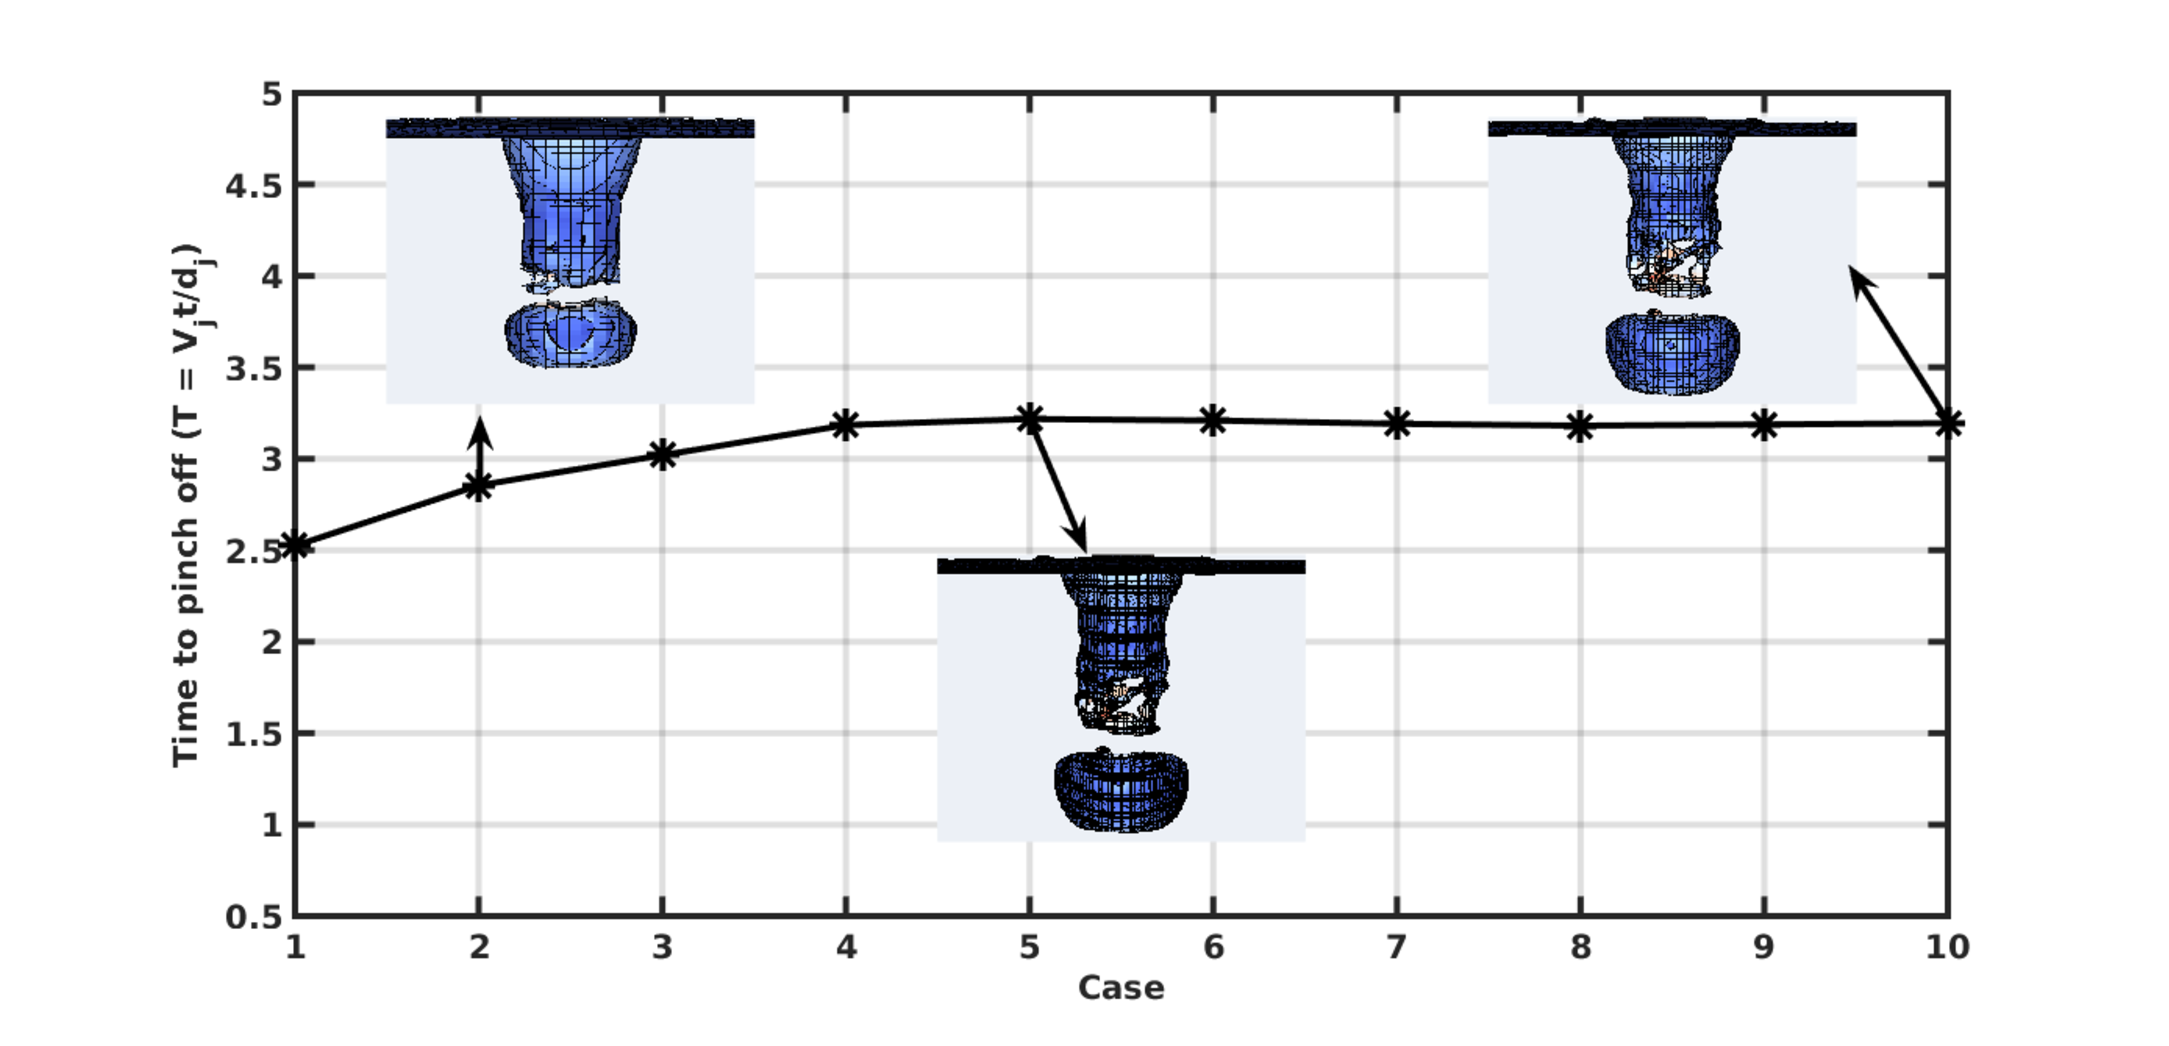
\includegraphics[width=\linewidth]{chapters/jetPool/Figure4}
	\caption{Determination of time taken for pinch off of first bubble after impact on the pool. The in-box figures represent instant of the pinch off. The $Fr_DFr_L  = 1.4 $ and $Re = 8000$ are kept constant. Interfacial grids obtained by full Adaptive Mesh Refinement (AMR) are shown in the inset corresponding to case 2 with a relatively coarse grid as well as in case 5 and case 10 with fine grids.}
	\label{Figure::GIS}
\end{figure}
\begin{figure}
	\centering
	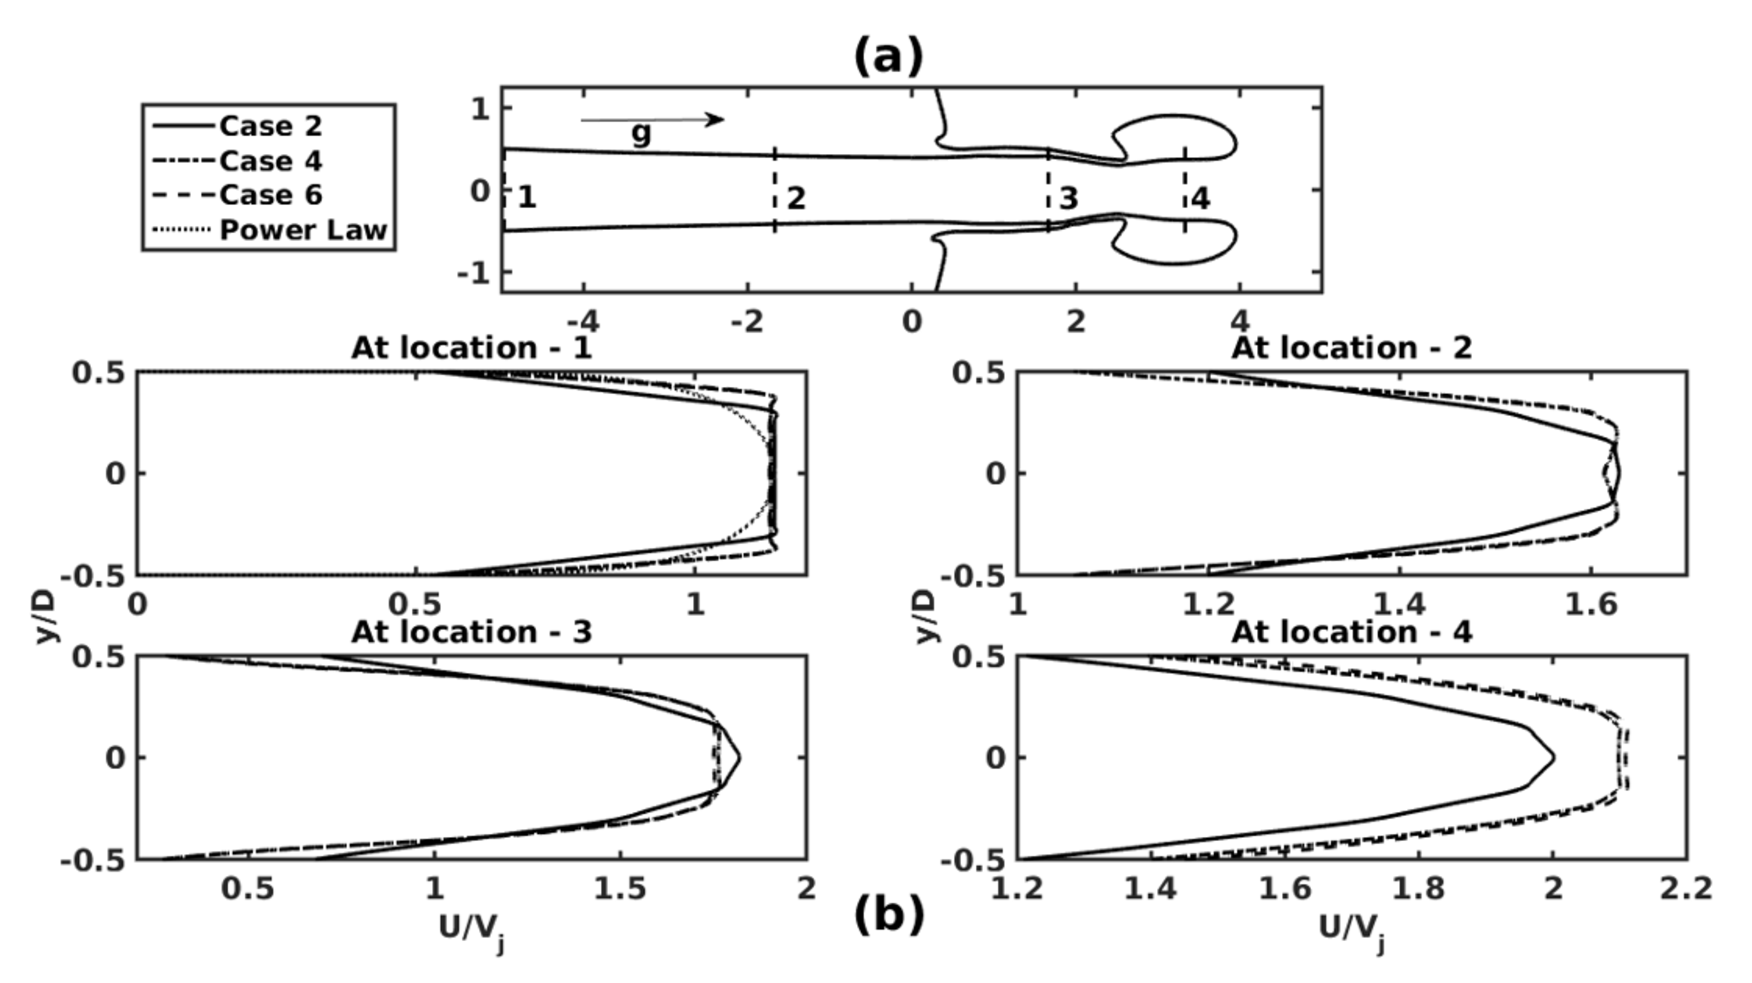
\includegraphics[width=\linewidth]{chapters/jetPool/Figure5}
	\caption{(a) Schematic of the different locations where the velocity profile is plotted and compared. The phase boundary corresponds to that of case 6. (b) Velocity profile as observed at indicated locations. ($Fr_DFr_L = 1.4$ and $T = \frac{V_jt}{d_j} = 2.5$)}
	\label{Figure::gisvel}
\end{figure}
\begin{table}
	\centering
	\begin{tabular}{@{}ccc@{}}
		\toprule
		Case  &\begin{tabular}[c]{@{}c@{}} $\: \: \: \: \: \: \: \: \: \left(\frac{d_j}{\delta l}\right)_{max}$ \end{tabular} & \begin{tabular}[c]{@{}c@{}} $\: \: \: \: \: \: \: \: \: \left(\frac{t_{CPU}}{t_{actual}}\right)$ \\ $\: \: \: \: \: \: \: \: \:$(days/s) \end{tabular}\\ \midrule
		4 & 51.2 & $\sim 7.5$\\
		5 & 102.4 & $\sim 10$ \\	
		6 & 204.8 & $\sim 15.5$ \\	\bottomrule
	\end{tabular}
	\caption{CPU performance data for simulations done for the Grid Independence Study. The simulations are done using four Intel Core i7-6500U CPU having clock speed of 2.5GHz each and 8 GB RAM.}
	\label{Table::cpu}
\end{table}
Figure~\ref{Figure::gisvel} shows the velocity profile at different locations across the jet, out of which location 1 is very near to the boundary where power law velocity profile has been patched (as described earlier in the mathematical formulation). Downstream to this, point 2 lies outside the liquid pool and has a fully developed water jet with high magnitude of velocities near the periphery where the air is present. A part of jet's initial gravitational potential has been converted into its kinetic energy resulting in higher velocity and lower instantaneous diameter. Other points are inside the pool with location 3 in the region surrounded by the thin air sheathe whose small velocity is reflected near the interface of the jet. Though the jet is inside the pool, it still retains its identity (with a lower velocity than expected due to impact with the pool) and after the pinch-off of the first bubble, jet continues to entrain bubbles inside the pool. Finally, location 4 is in the liquid region of the first annular bubble that pinches off. Figure~\ref{Figure::gisvel} clearly demonstrates that the velocity profile is independent of spatial refinement beyond case 4, justifying the approach to select the mesh parameters of case 5 as the fundamental configuration.
\subsection{Validation of the numerical code}
\begin{figure}
	\begin{minipage}{0.5\linewidth}
		\centering
		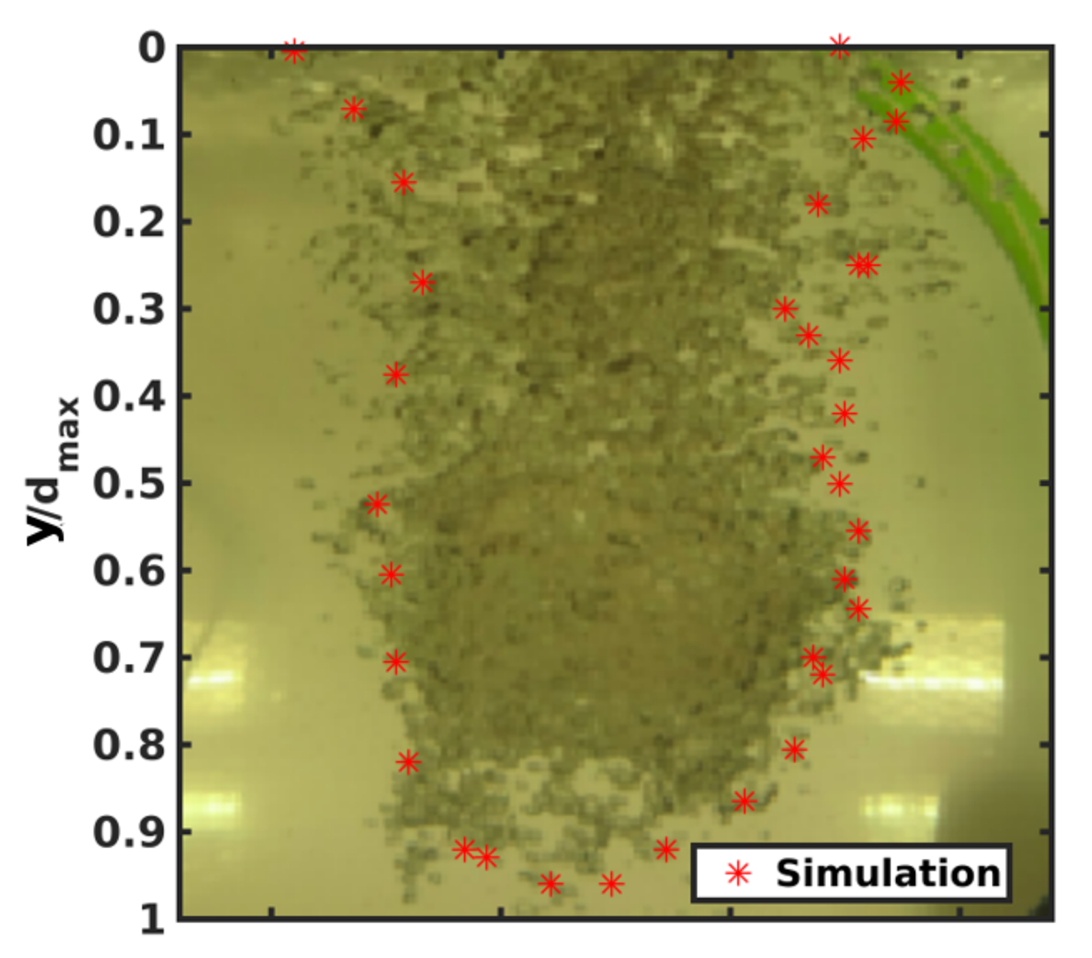
\includegraphics[width=\linewidth]{chapters/jetPool/Figure6a}
		(a)
	\end{minipage}
	\begin{minipage}{0.5\linewidth}
		\centering
		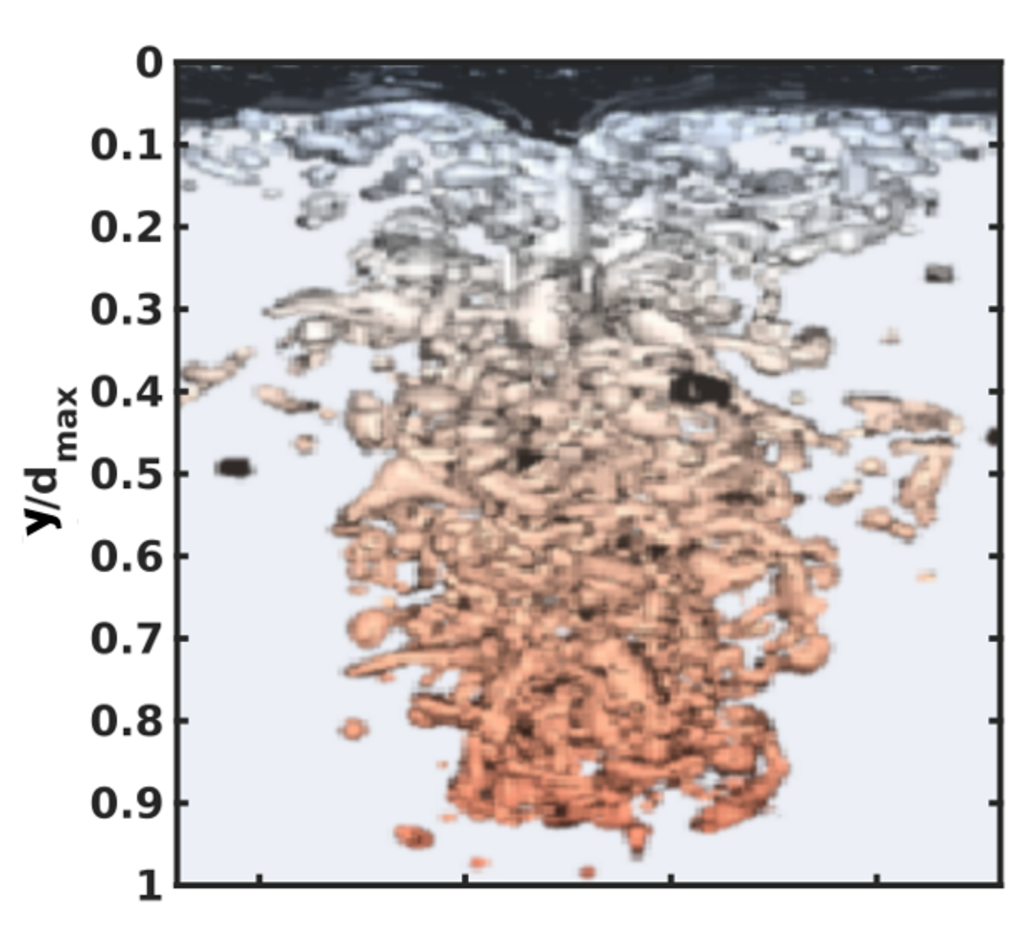
\includegraphics[width=\linewidth]{chapters/jetPool/Figure6b}
		(b)
	\end{minipage}
	\caption{(a) Experimental snapshot of the bubble cluster below the liquid pool with points of the interface obtained from numerical simulation (b) Numerically obtained bubble cluster at $Fr_DFr_L$ = 1.4; both experimental snap and numerical contours are plotted at T = 300 starting from jet touching the pool.}
	\label{Figure::valid}
\end{figure}
\begin{figure}
	\centering
	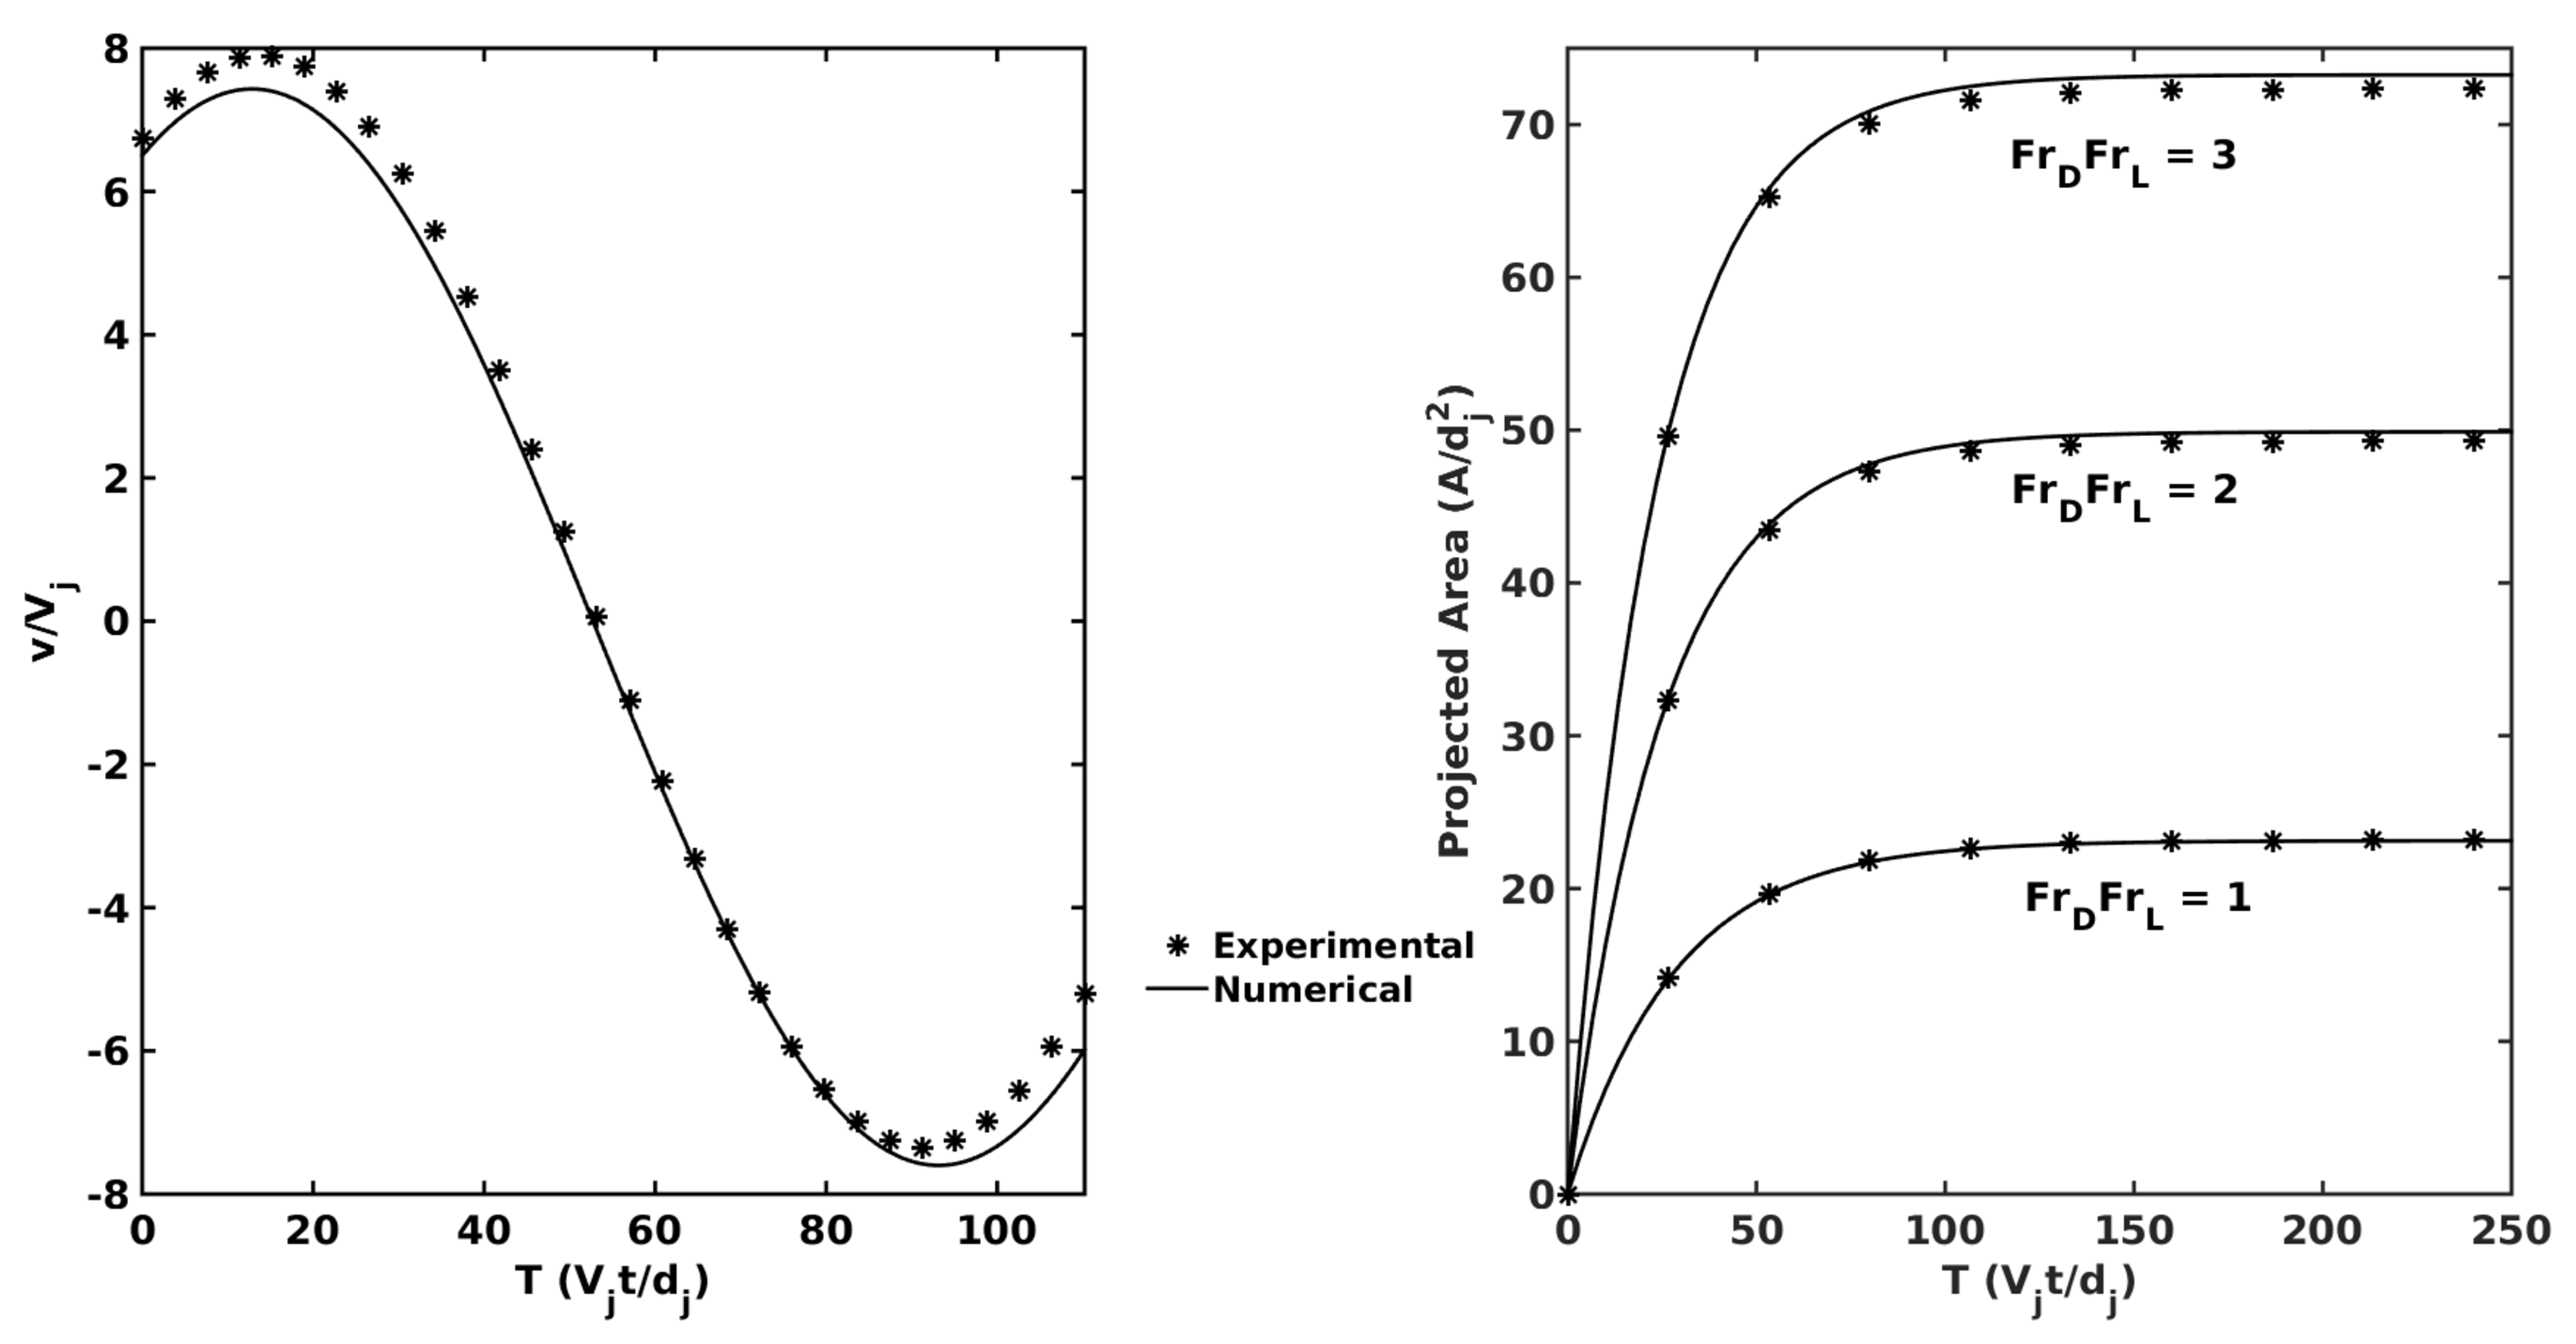
\includegraphics[width=\linewidth]{chapters/jetPool/Figure7}
	\caption{Comparison between experimental and numerically obtained results for temporal variation of (a) Velocity vector of a typical bubble in the entrained region at $Fr_DFr_L$ = 1.8 (b) Projected area of the entrained bubble cluster }
	\label{Figure::valid2}
\end{figure}
Next, the numerical code employed is tested for its validity by virtue of its correspondence with the experimental observations. Figure~\ref{Figure::valid} contains the results of validation test carried out for $Fr_DFr_L = 1.4$. The numerically simulated interface structure shows a remarkable similarity with the experimentally obtained bubble cluster interface. Velocity variation of a bubble in the cluster with time is obtained from experimental snaps and reported in figure~\ref{Figure::valid2} (a) along with data of a bubble from a numerical simulation. A close match between numerical prediction and experimental observation validates the developed model. Moreover, efforts are also made to measure the area occupied by the bubble cluster from temporal snaps of experimental observation. Development of cluster area with time from the experiment is plotted in figure~\ref{Figure::valid2} (b) along with numerical findings. It can be observed from the figure that experiment and numerical simulation corroborates similar observations for a range of $Fr_DFr_L$.
Next section illustrates the two possible outcomes of the jet-pool interactions, no entrainment, and vigorous bubble cluster formation. These are obtained from experimental snapshots. 

\section{Continuous and no entrainment}
\begin{figure}
	\centering
	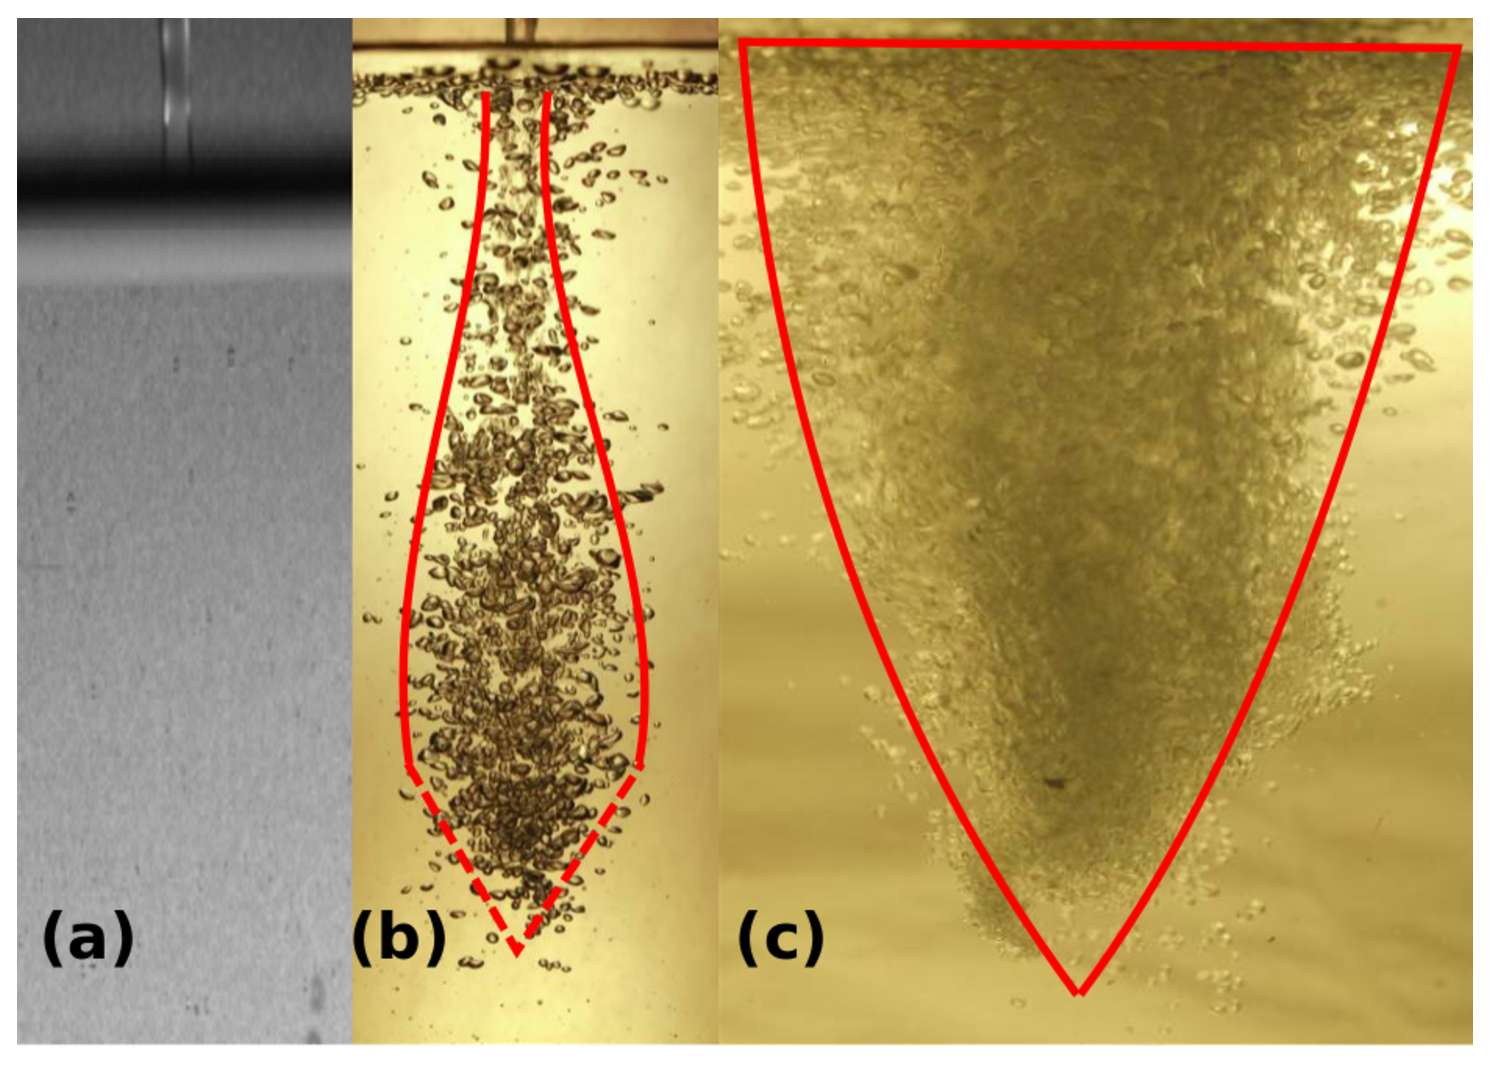
\includegraphics[width=0.75\linewidth]{chapters/jetPool/Figure8}
	\caption{Possible outcomes as the jet impinges onto the pool: (a) No entrainment $Fr_DFr_L = 0.125$, (b) Continuous Entrainment with diverging converging cluster $Fr_DFr_L = 1.25$ and (c) Continuous Entrainment with triangular entrainment region  $Fr_DFr_L = 3.8$}
	\label{Figure::transition}
\end{figure}
Figure~\ref{Figure::transition} shows two types of possibilities when the liquid jet impinges the water surface. Even though, the inception of air bubble entrainment is not easily characterized.Experimental observation showed that for a low inertial jet, the flow is likely to be laminar and there is no air entrainment (figure~\ref{Figure::transition} (a)). With an increase of $Fr_DFr_L$, an air bubble cluster is observed below the impact point inside the test pool. In figure~\ref{Figure::transition} (b), at $Fr_DFr_L = 1.1$, a diverging-converging shape is observed. At even higher $Fr_DFr_L$, a triangular entrainment region is observed as shown in figure~\ref{Figure::transition} (c). The outer bound of the bubble cluster is shown in the figure with a red line. The depth of the cluster is observed to be varied as a function of jet inertia as discussed later on. The transition between entrainment and no entrainment is not well defined and is prompt \citep{Harby2014,ervine1980effect}. But it has been observed (discussed later) that entrainment height diminishes with $Fr_DFr_L$ and there exists a critical $Fr_DFr_L$ below which entrainment is not present. Assessment of this transition exactly in terms of $Fr_DFr_L$ is quite difficult which requires precise control of flow rate. The present experimental setup is not equipped with such precision and therefore focus has been kept on the entrainment regime. But, \citet{Harby2014} have defined inception of entrainment as the entry of more than three bubbles in the liquid pool in three minutes and proposed inception velocity as a function of $\frac{l_j}{d_j}$. These isolated efforts showing no entrainment falls well within the limit mentioned by \citet{Harby2014}. Based on present experimental efforts it can be ensured that for $Fr_DFr_L$ less than 0.1 will not show any entrainment. For precise limit, one may follow limits proposed by \citet{Harby2014}. Next, a subtle account of the onset of entrainment process is presented.
\section{Onset of entrainment}
\begin{figure}
	\centering
	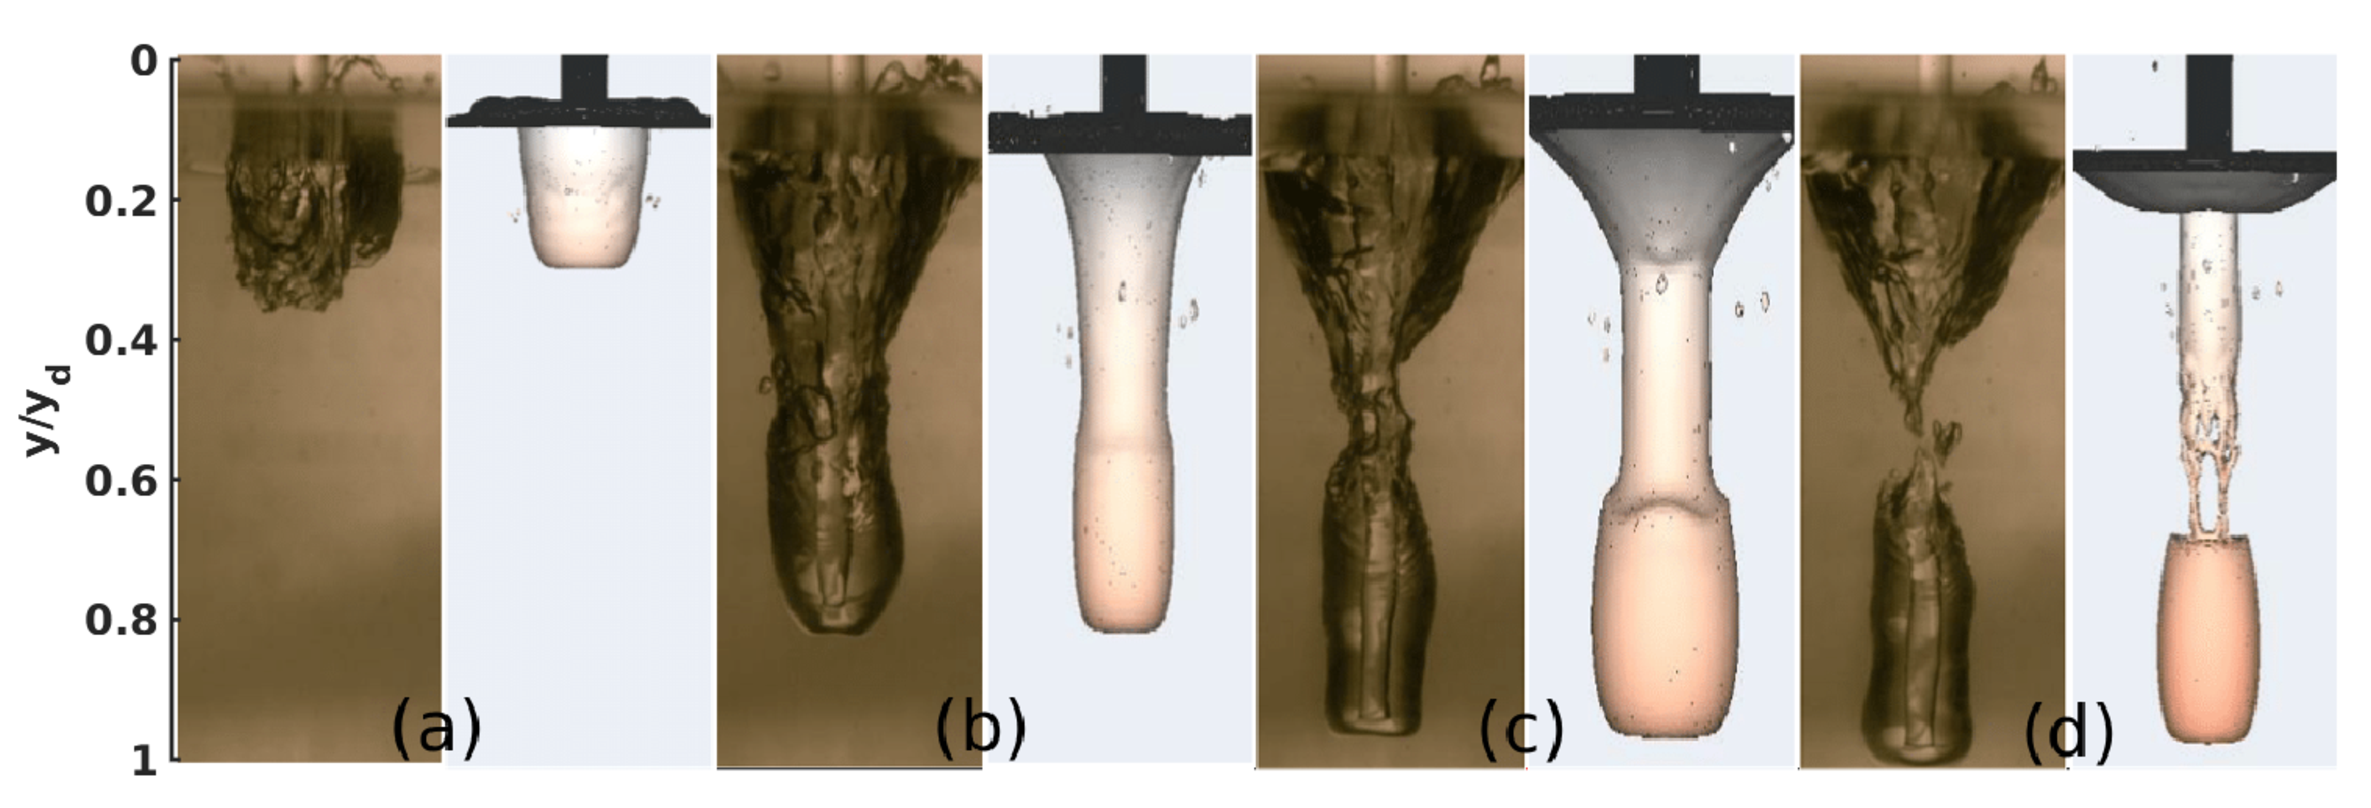
\includegraphics[width=\linewidth]{chapters/jetPool/Figure9}
	\caption{The temporal record of the onset of entrainment; (left: experimental and right: numerical) (a) Jet impacts the liquid pool and forms a cavity at $T = \frac{V_jt}{d_j} = 1$, (b) Elongation of the cavity formed at $T = 1.95$, (c) Necking of the elongated cavity at $T =2.5 $ as surface tension force tries to overcome jet's inertia and (d) Pinch off of the first annular air bubble at $T = 3.5$. ($Fr_DFr_L = 2.2$).}
	\label{Figure::pinchNum}
\end{figure}
To understand the two opposite possible outcomes mentioned above, the onset of entrainment is observed. Onset will be propagated or suppressed to reach either in the no entrainment or continuous entrainment scenario, respectively.
\subsection{Pinch-off of first annular bubble}
Figure~\ref{Figure::pinchNum} consists of a detailed account of the jet - pool interaction from the point of impact to the point of pinch off. Both experimental snapshots and numerical tracer contours are shown side by side to establish the onset dynamics. As the jet strikes the liquid pool, a cavity is formed with the liquid core at the centerline surrounded by the air medium which by virtue of inertia penetrates inside resulting in the formation of a long cylinder. Surface tension and circulation surrounding the jet (as discussed later) results in necking which propagates further and pinches off as shown in figure~\ref{Figure::pinchNum} (d). The process has been studied from high-speed images in detail for the onset of entrainment for $Fr_DFr_L = 1$ (figure~\ref{Figure::pinchex}). It can be observed from experiments that upon striking the free surface, due to inertia, jet creates a dimple and propagates downwards to form a cavity filled with air (figure~\ref{Figure::pinchex} (a)). With time, the cavity enlarges (figure~\ref{Figure::pinchex} (b) - \ref{Figure::pinchex} (e)) before surface tension becomes significant and starts contracting the cavity back to its original free surface. In the initial period, air cavity is formed as stepped cylinder with continuously decreasing diameter (figure~\ref{Figure::pinchex} (a) - \ref{Figure::pinchex} (c)). \\
\begin{figure}
	\centering
	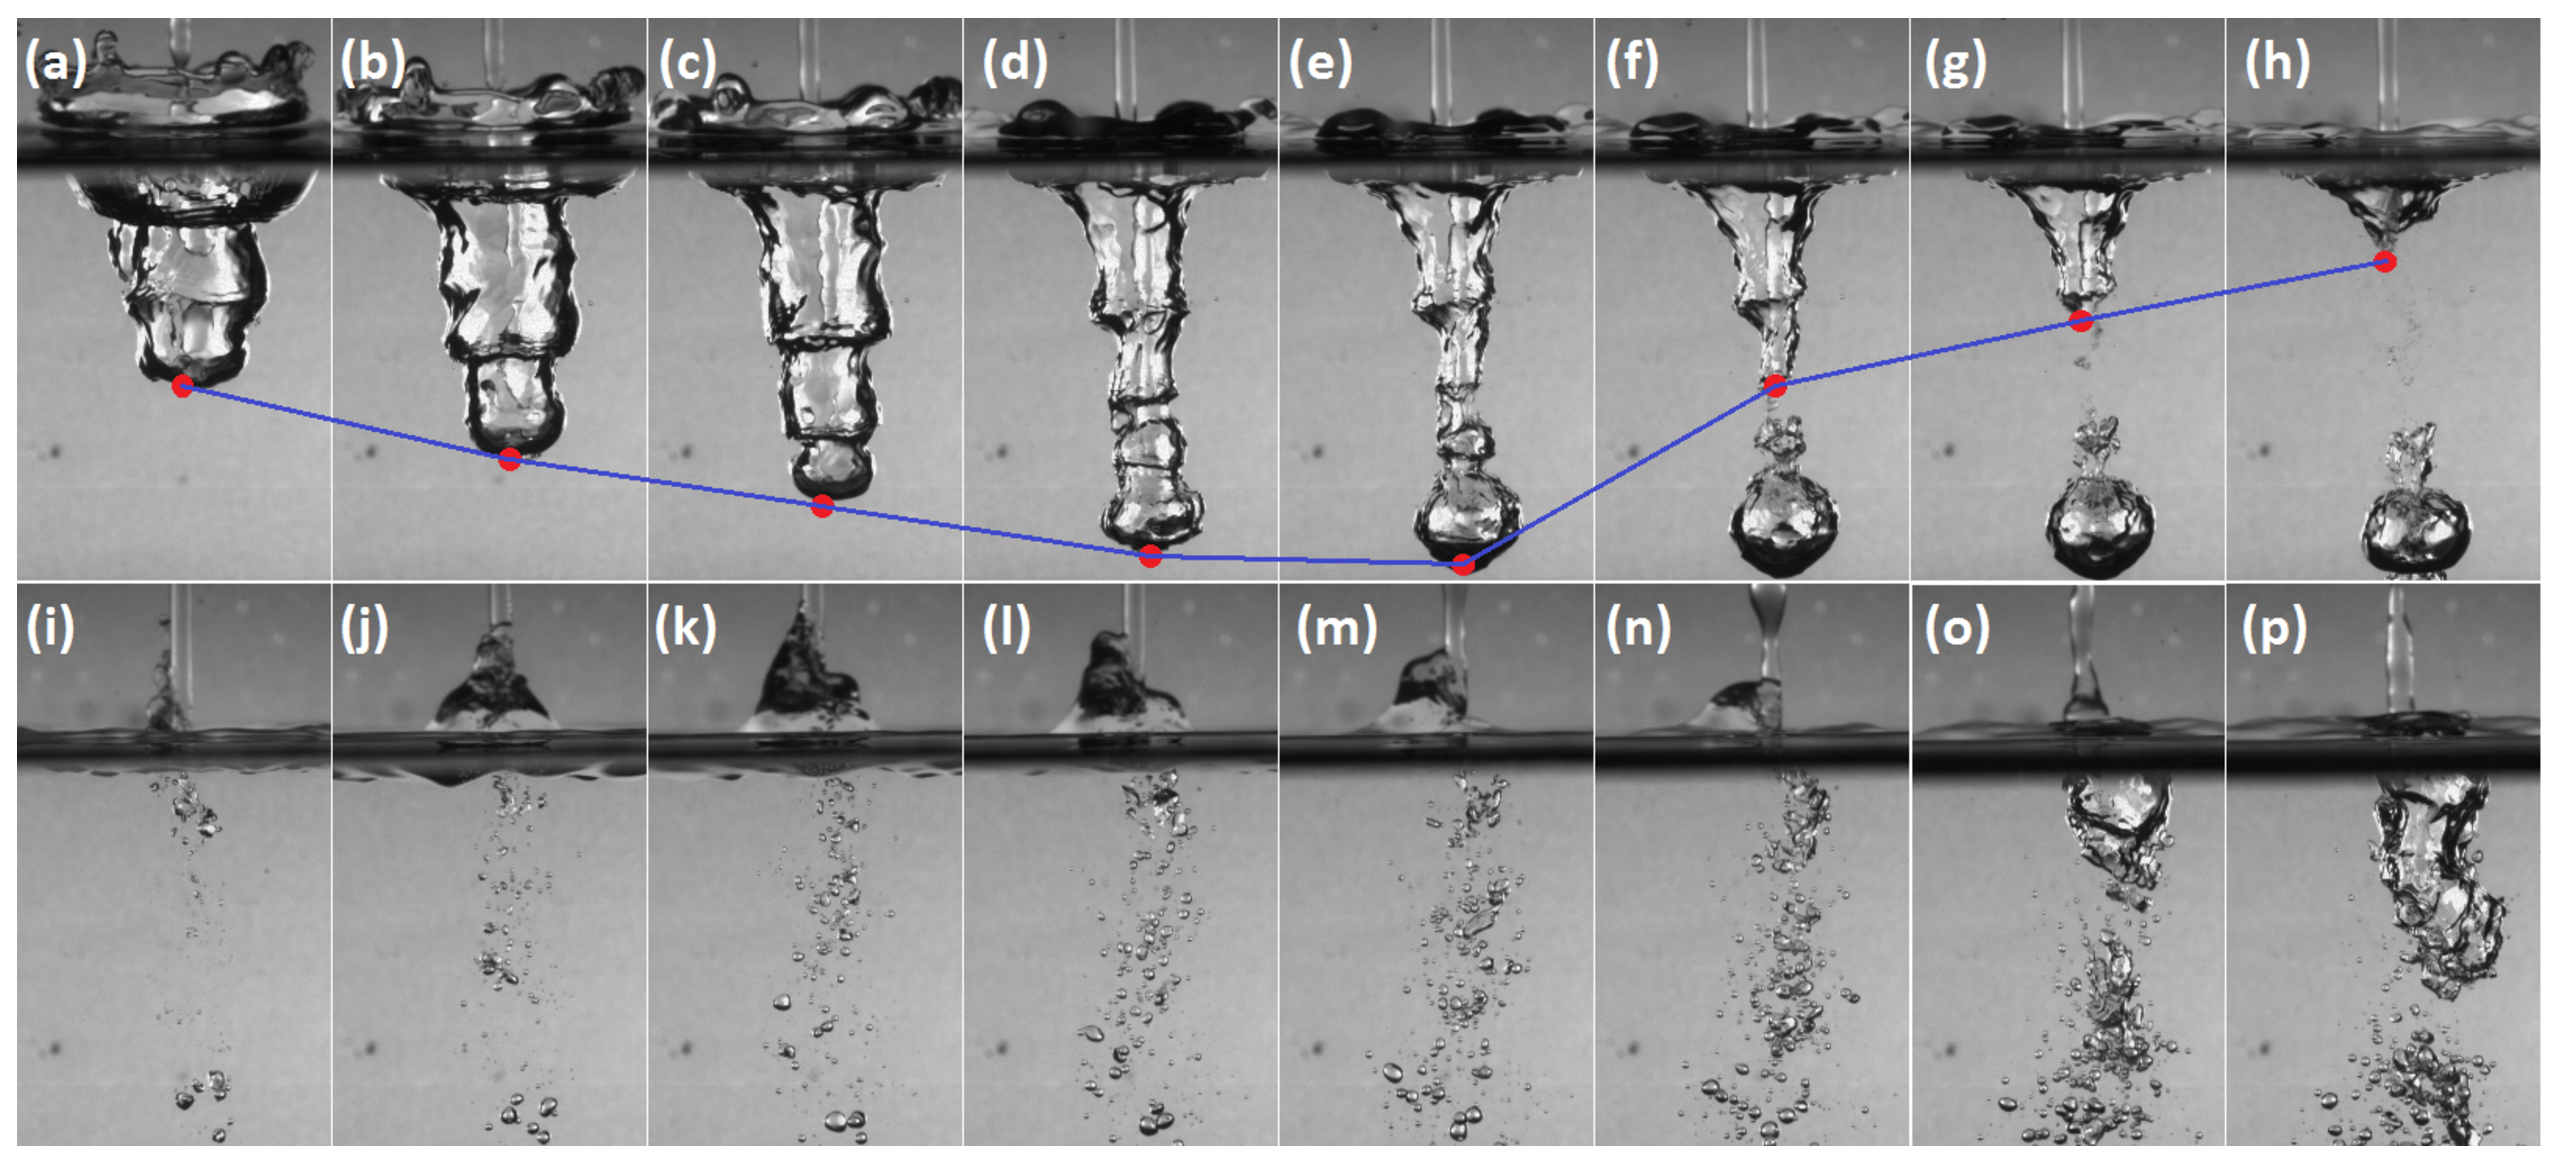
\includegraphics[width=\linewidth]{chapters/jetPool/Figure10}
	\caption{Experimental snapshots of pinch off for $Fr_DFr_L = 1$  at $T = $ (a) $2.04$, (b) $2.28$, (c) $2.52$, (d) $2.76$, (e) $2.88$, (f) $3$, (g) $3.24$, (h) $3.35$, (i) $3.5$, (j) $3.75$, (k) $4$, (l) $4.25$, (m) $4.5$, (n) $5$, (o) $5.5$ and (p) $6$}
	\label{Figure::pinchex}
\end{figure}
At a critical depth, surface tension starts dominating and cylinder turns into a sphere (figure~\ref{Figure::pinchex} (d)) to initiate the contraction of the cavity. At this level, inertia gets weakened and surface tension starts dominating. Due to conversion of cylindrical cavity into spherical air mass (figure~\ref{Figure::pinchex} (e)), pressure waves are generated which propagates in upward direction and contracts the stepped cylinder towards the jet (figure~\ref{Figure::pinchex} (e) - \ref{Figure::pinchex} (f)), prompting collapse of the cavity. While the cavity is being collapsed, spherical air mass at the bottom of the cavity forms neck (figure~\ref{Figure::pinchex} (e)) as a result of the higher amplitude of three-dimensional pressure waves. This leads towards pinching (figure~\ref{Figure::pinchex} (f)) off the spherical bubble along with some satellites and retraction of rest cavity towards the free surface (figure~\ref{Figure::pinchex} (f) - \ref{Figure::pinchex} (h)). The experiment shows that collapse of cavity generates an upward moving liquid jet (figure~\ref{Figure::pinchex} (i)) thicker than the impinging one (figure~\ref{Figure::pinchex} (j)). These two counteracting jets entrap air bubble in between them (figure~\ref{Figure::pinchex} (k)). As the velocity of impinging jet is higher than the pressure wave jet, entrapped bubbles move down in the pool (figure~\ref{Figure::pinchex} (k) - \ref{Figure::pinchex} (l)). With time, jet created by pressure wave falls down (figure~\ref{Figure::pinchex} (m) - \ref{Figure::pinchex} (n)) and impinging jet starts second cycle of cavity formation (figure~\ref{Figure::pinchex} (o)). The whole process repeats many times to entrap more and more bubbles (figure~\ref{Figure::pinchex} (p)) and finally form a cluster as shown in experimental observation of figure~\ref{Figure::transition} (c). The detached spherical bubble in each cycle comes back to the free surface and in its path, it dislodges daughters due to impact from bubbles in the cluster. At a lower value of the product of Froude numbers ($Fr_DFr_L$), inertia never becomes dominated over surface tension and gravitational collapse strength to show all these sequences for the formation of the bubbly cluster. Impingement of jet at lower $Fr_LFr_D$, creates a cavity but its propagation in the downward direction is suppressed and immediate collapse causes no entrainment of bubbles. But this requires further proof in future efforts.\\
\begin{figure}
	\centering
	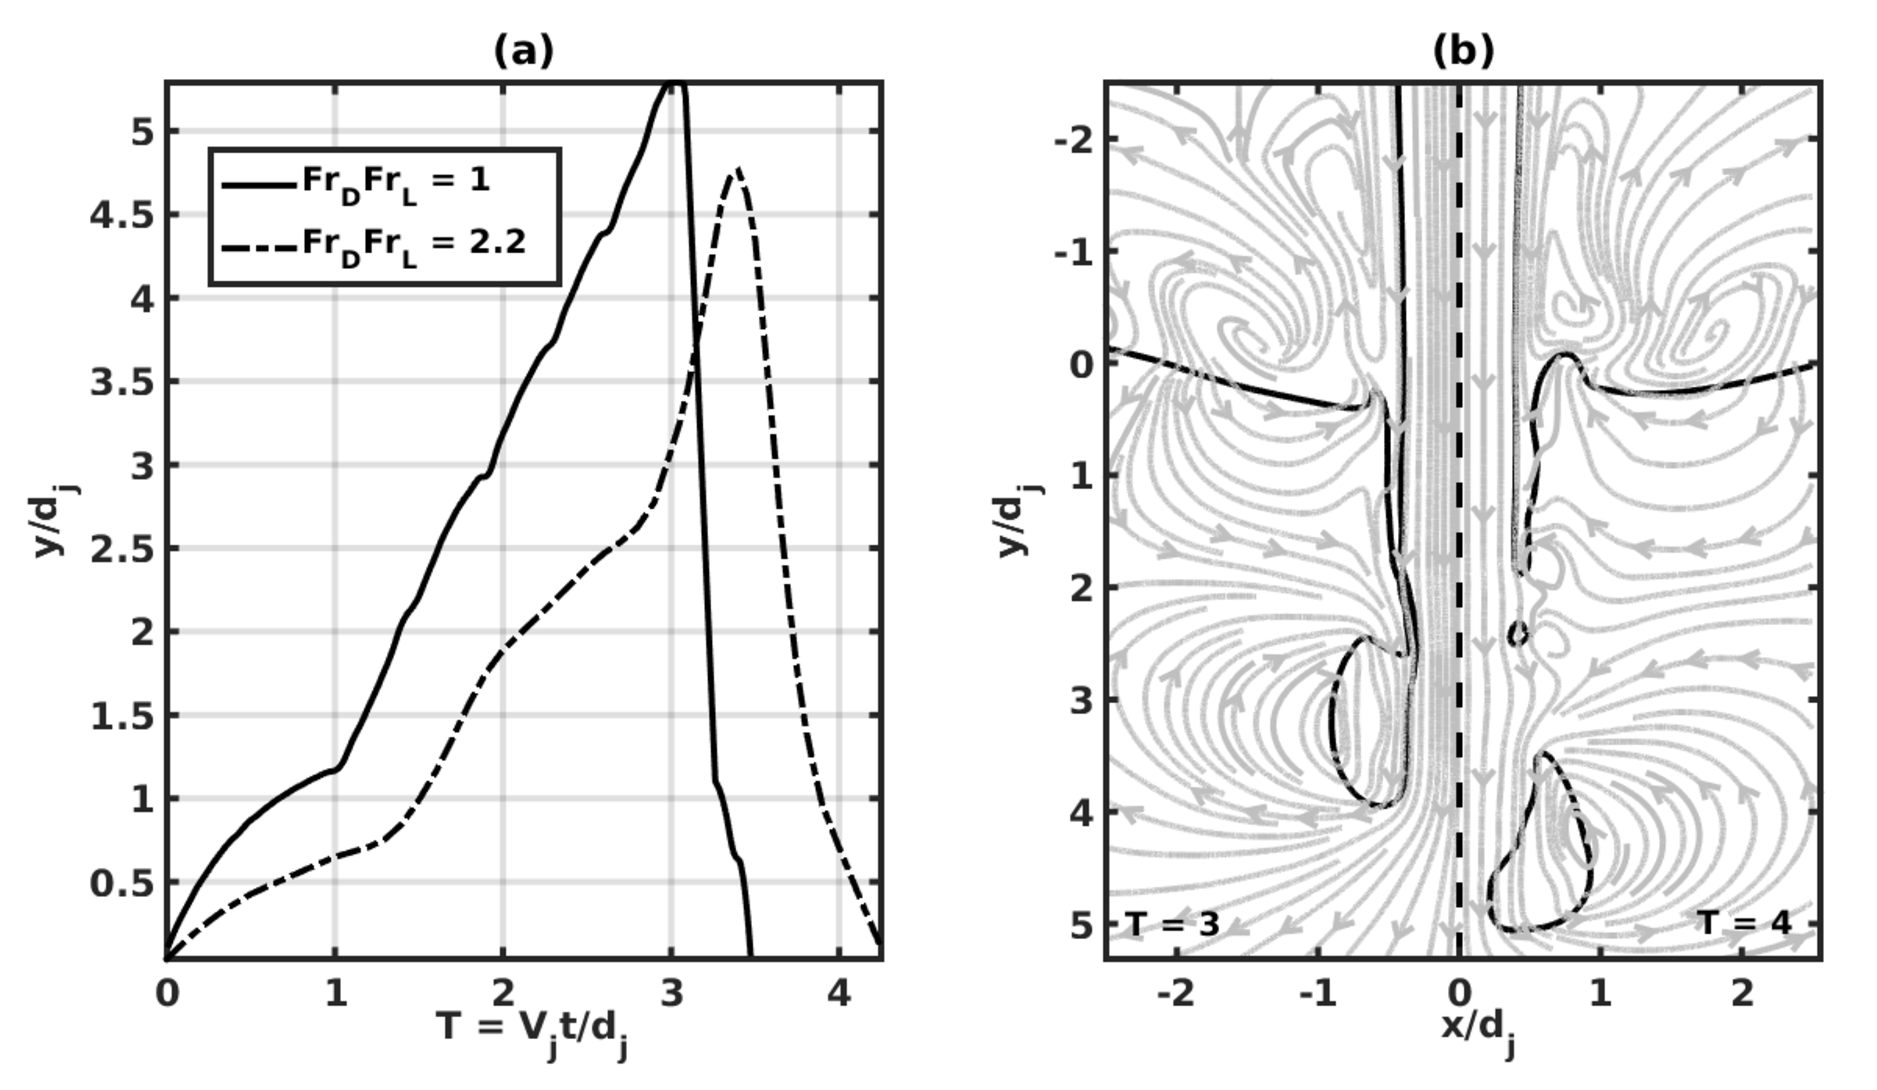
\includegraphics[width=\linewidth]{chapters/jetPool/Figure11}
	\caption{(a) Depth of penetration of liquid cavity formed during the impact of jet onto the pool and subsequent collapse of cavity. (b) Streamlines developed around the formed cavity before (on left) and after (on right) pinch off.}
	\label{Figure::stream}
\end{figure}
\subsection{Dynamics of first pinch-off}
One can clearly understand from the high-speed image sequences of figure~\ref{Figure::pinchex} that during onset, the cavity collapses (surface tension driven) at a faster rate than formation (inertia dominated). Figure~\ref{Figure::stream} (a) shows the maximum depth of the cavity with time as obtained from numerical simulations, for a complete cavity cycle. Initially, depth increases at a slower rate till pinch off of the bubble, as represented by steep fall in depth. Subsequently, the collapse of cavity occurs at a faster rate as shown in figure~\ref{Figure::stream} (a). With the streamline field in figure~\ref{Figure::stream} (b) obtained through numerical simulations, the dynamic process of pinch-off is studied. As the cylindrical cavity elongates (by virtue of jet's inertia) the surrounding air-sheathe gets thinner and a region of high circulation is realized around the jet. As the jet tries to further elongate the cavity against the resistance of the pool, the developing circulations catapult the bubble and pinches it off from the thin air sheathe. A look at the streamlines near the pool surface justifies the movement of the point of pinch-off towards the incoming jet as the cavity collapses back. As the cycle repeats, more bubbles are entrapped which ultimately leads to the formation of bubble cluster below the surface. Next, dynamic nature of the generated bubble cluster and characterize it based on the strength of the jet are illustrated.
\section{Dynamics of bubble cluster}
In two-phase chemical reactors, the rate of reaction often depends on the available surface area in form of interfaces. Formation of bubbles inside the liquid pool increase this interfacial area and is responsible for the transfer of mass and energy through diffusion and advection. Therefore, it is pertinent to realize the characteristics of these bubble populations. The interaction between bubbles includes collision, coalescence, and dissociation. These processes lead to the formation of the bubble cluster which can be treated as a unique body whose dimensional characteristics are germane to the design of chemical reactors.
\subsection{Attainment of quasi-steady bubble cluster}
\begin{figure}
	\centering
	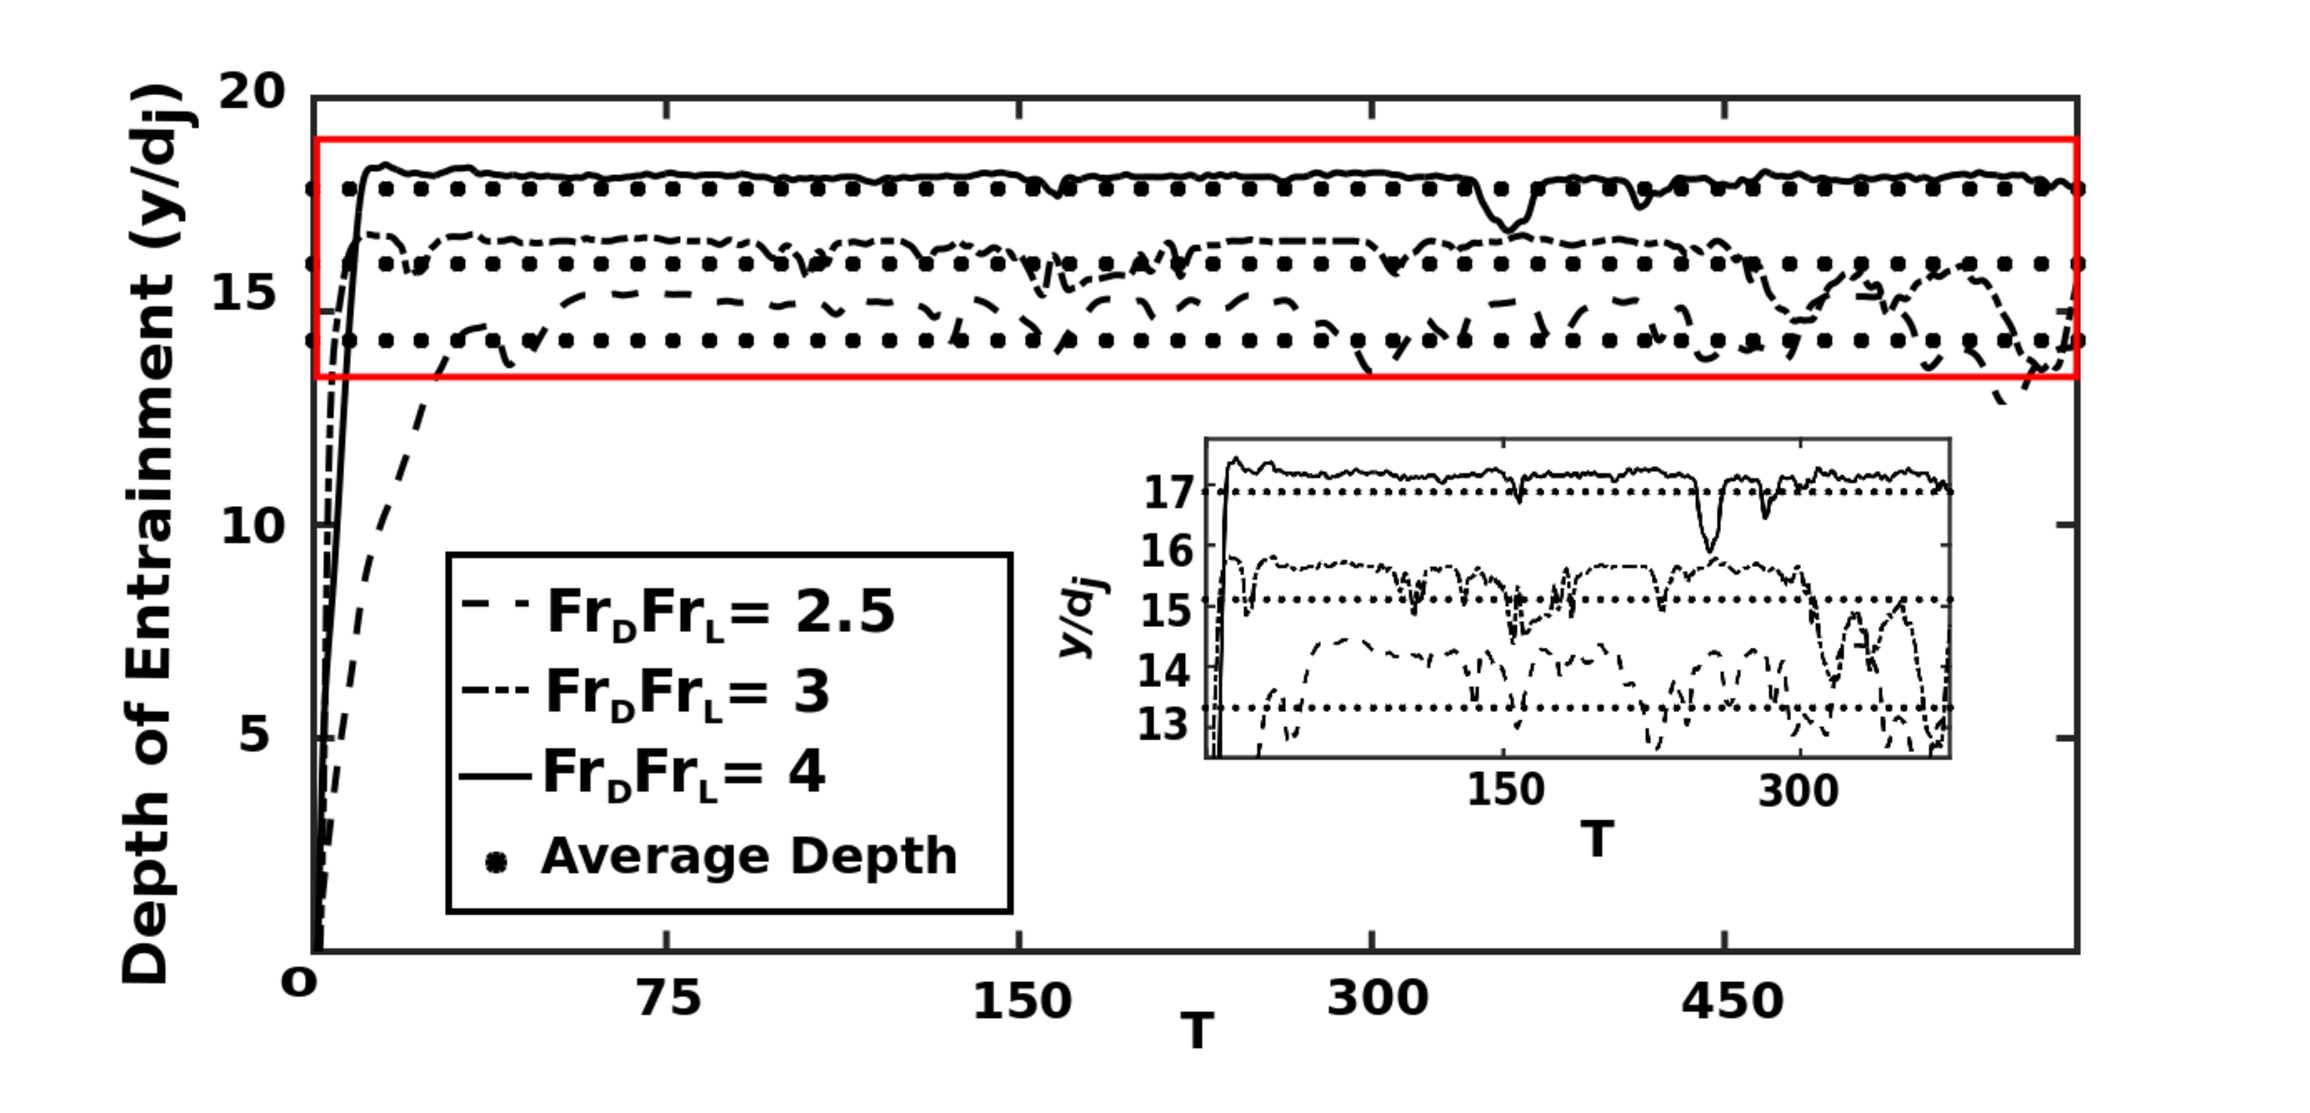
\includegraphics[width=\linewidth]{chapters/jetPool/Figure12}
	\caption{Temporal variation of maximum depth of entrainment. The inset figure takes a closer look at the variation of the height of entrainment, which pertains to a nearly constant value.}
	\label{Figure::TemporalHeight}		
\end{figure}
Once the cluster of different sized, shaped and interacting bubbles comes into existence, dynamics of an individual bubble is hard to follow. Overall nature of the bubble cluster remains almost same and the depth of entrainment attains a steady state value. In figure~\ref{Figure::TemporalHeight}, from experimental observations, the variation of the depth of entrainment with time for different strengths ($Fr_DFr_L$) of the jet is shown. Experimentally, after onset (increasing depth with time), saturation of depth is observed up-to a prolonged period. For different jet strengths, the average depth (with dots) which is in the range of saturation is also plotted. It shows that after onset, depth of entrainment is not a function of time, rather depends on the strength of the impinging jet. This nature has been shown clearly in the inset of figure~\ref{Figure::TemporalHeight}.
\begin{figure}
	\centering
	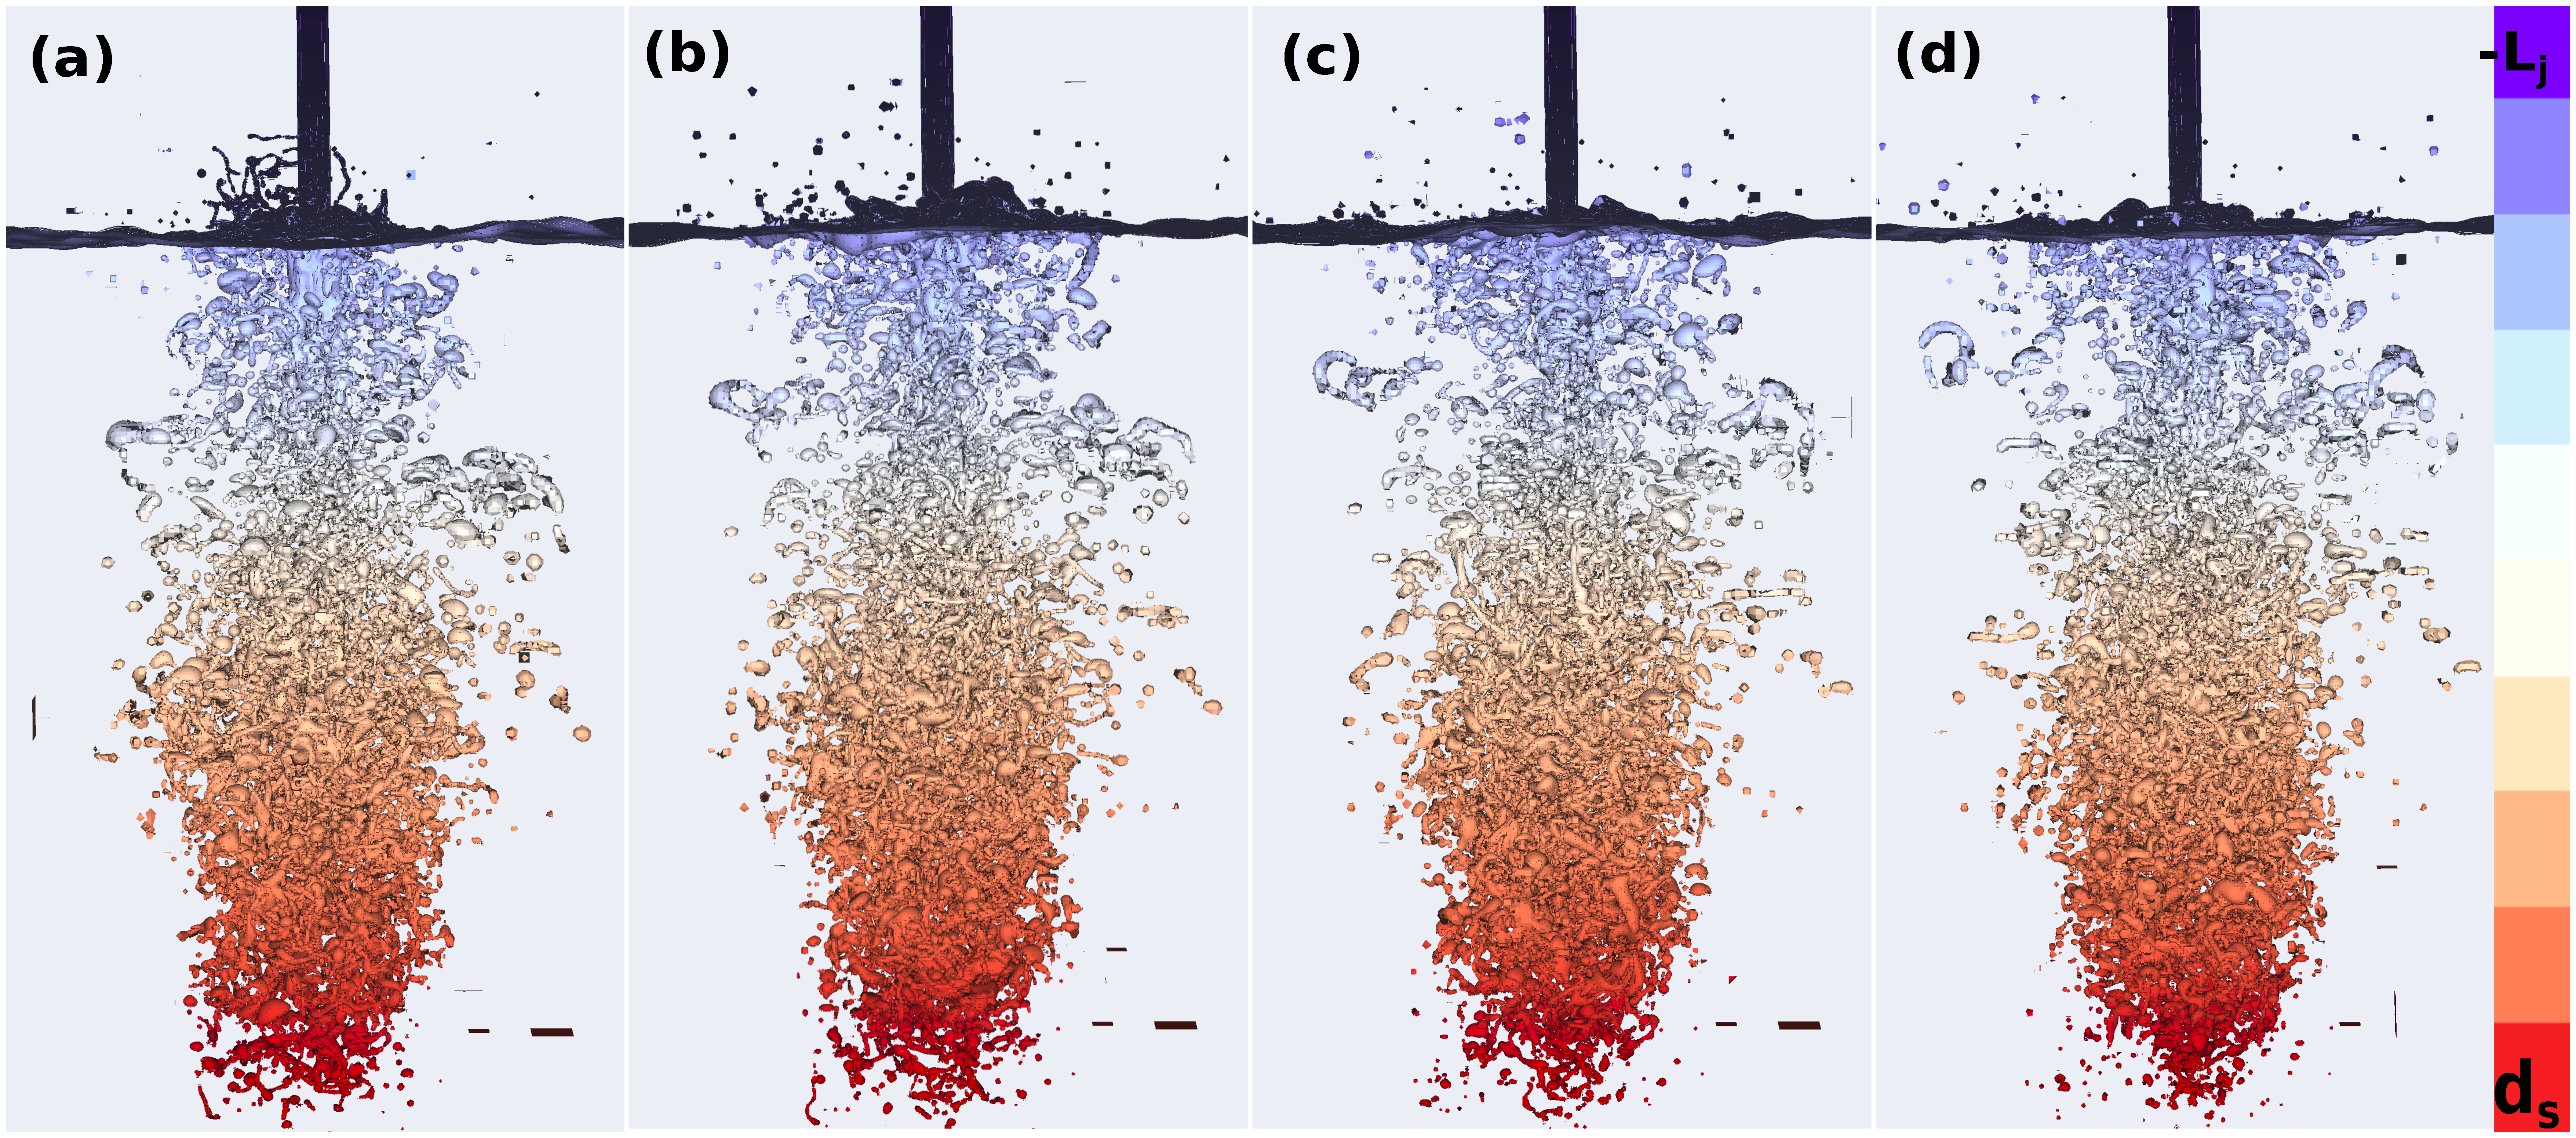
\includegraphics[width=\linewidth]{chapters/jetPool/Figure13}
	\caption{Attainment of steady state entrainment height for $Fr_DFr_L$ = 4 with the interface colored by the depth as measured from the liquid pool interface at $T =$  (a) $85$, (b) $90$, (c) $95$ and (d) $100$}
	\label{Figure::hsteady}		
\end{figure}
\begin{figure}
	\centering
	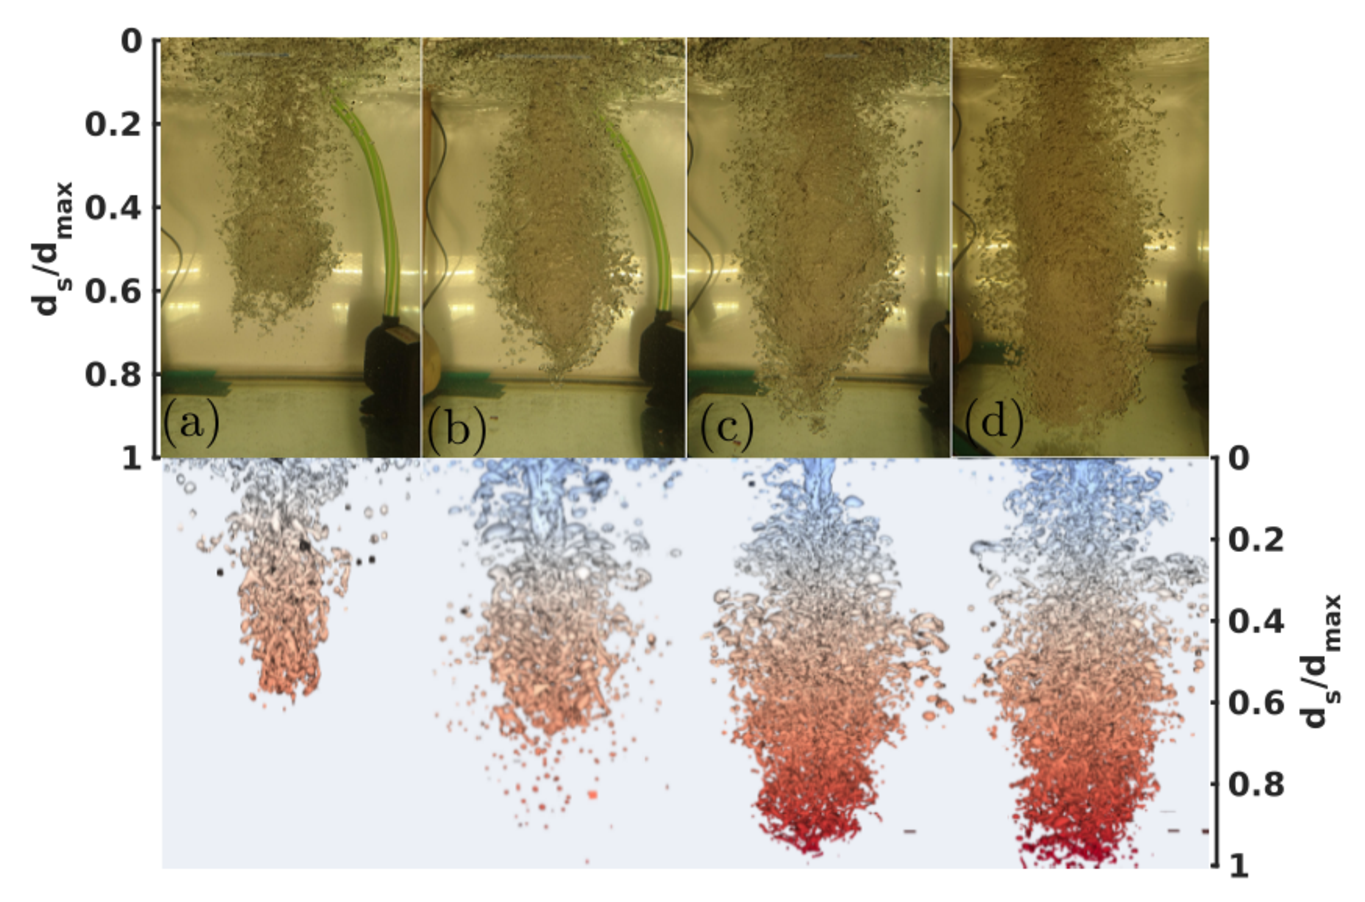
\includegraphics[width=\linewidth]{chapters/jetPool/Figure14}
	\caption{Steady entrainment pattern for  $Fr_DFr_L$ = (a) 1.4, (b) 2, (c) 3.25 and (d) 3.75}
	\label{Figure::height_diff}		
\end{figure} 
\subsection{Characterization of bubble cluster}
Steady penetration of entrainment inside pool is also confirmed by numerical simulations. In figure~\ref{Figure::hsteady}, detailed Volume of Fluid tracer colored using the distance from the liquid pool interface as the scalar has been shown. Numerical simulation shows that the depth of penetration of the bubble cluster pertains to a constant value as the time passes. Present numerical simulation matches well with the experimental observation here. In figure~\ref{Figure::TemporalHeight}, experimentally, an increase of steady depth for three $Fr_DFr_L$ is observed. Experimental and numerical snapshots of entrainment pattern at different $Fr_DFr_L$ are shown in figure~\ref{Figure::height_diff} to confirm the story of interface locations. From these photographic observations and numerical phase contours, one can observe that the entrained air penetration depth is proportional to $Fr_DFr_L$. A complete range of depth ($d_s$) variation of entrainment from the free surface for a wide range of $Fr_DFr_L$ is shown in  figure~\ref{Figure::hFr}. Both experimental and numerical data points are shown in figure~\ref{Figure::hFr}. To express this increasing pattern of cluster depth as a function of $Fr_DFr_L$, correlations (equation~\ref{Equation::fitlinear1} for $log(Fr_DFr_L) < 1.2$ and equation~\ref{Equation::fitlinear2} for $log(Fr_DFr_L) > 1.2$ ) with two empirical constants each in the form of a power law are proposed. The change in the behavior of the curves is because of the difference in entrainment cluster regimes as observed in figure~\ref{Figure::transition}. The empirical constants are fitted from experimental observations with Summed Square of Residue (SSE) equal to 7.5 X $10^{-2}$ and 5 X $10^{-2}$ and R-square value as $0.9$ and $0.95$ respectively for equation~\ref{Equation::fitlinear1} and~\ref{Equation::fitlinear2}. 
\begin{equation}
\frac{ds}{dj} = 9.45(Fr_DFr_L)^{0.33}
\label{Equation::fitlinear1}
\end{equation}%
\begin{equation}
\frac{ds}{dj} = 3.3(Fr_DFr_L)^{1.2}
\label{Equation::fitlinear2}
\end{equation}%
\begin{figure}
	\centering
	\includegraphics[width=\linewidth]{chapters/jetPool/Figure15}
	\caption{Steady state depth of entrainment as a function of the product of Froude numbers, $Fr_DFr_L$; both experimental and numerical data points are mentioned.}
	\label{Figure::hFr}
\end{figure}
\begin{figure}
	\centering
	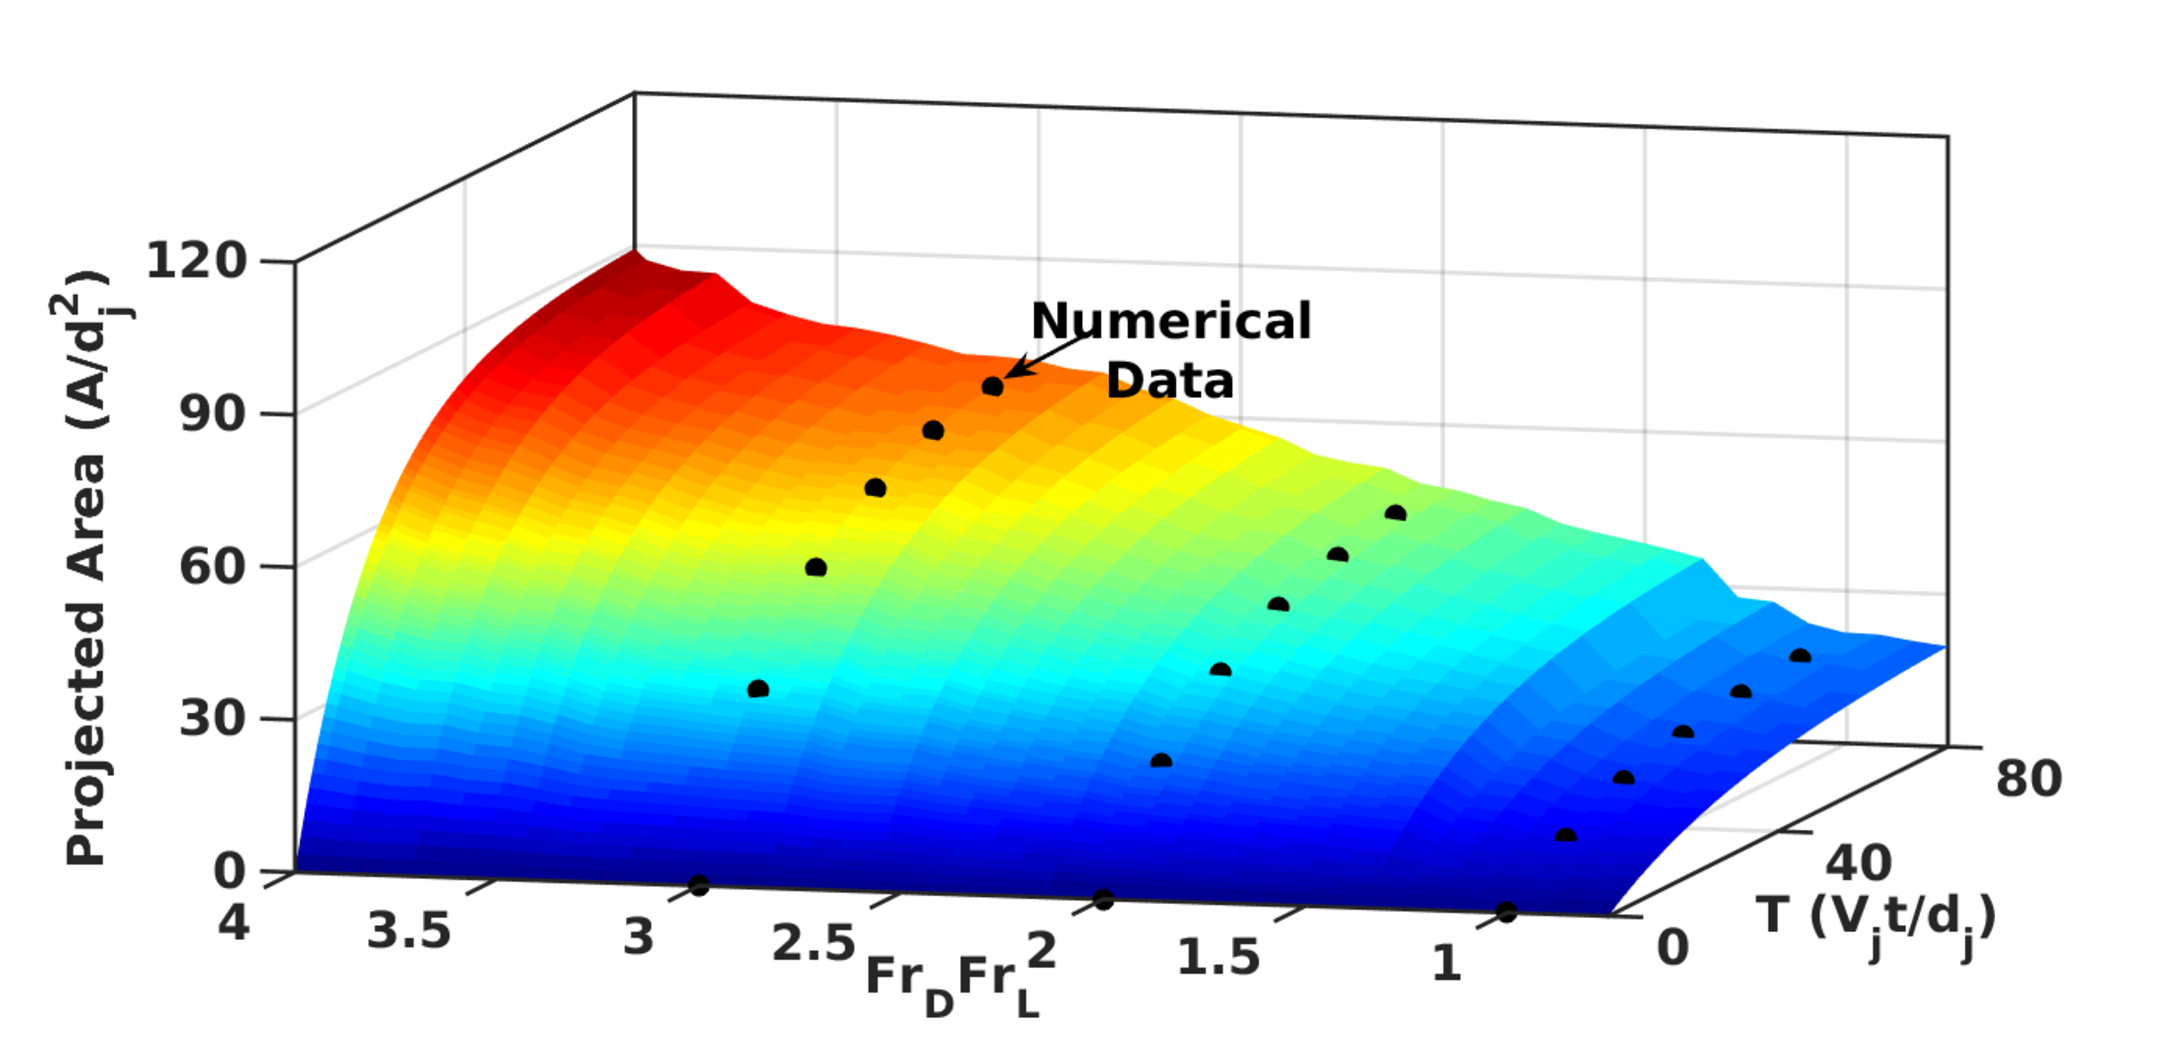
\includegraphics[width=\linewidth]{chapters/jetPool/Figure16}
	\caption{Projected area of the region affected by entrained bubble cluster; plane is constructed by experimental observations and numerical data points are shown by symbols.}
	\label{Figure::area}
\end{figure}
To show the predictability of already available correlations against the experimental observations and establishment the improvement in prediction using equation (\ref{Equation::fitlinear1}-\ref{Equation::fitlinear2}), power law as proposed by \citet{ohkawa1986some} is also shown in Figure~\ref{Figure::hFr}.
Further, the volumetric strength of bubble cluster has been also observed to change with jet strength ($Fr_DFr_L$) in Figure~\ref{Figure::height_diff}. The variation of the projected area of the cluster in a two-dimensional photographic plane along with the time at different jet strength is given. In Figure~\ref{Figure::area}, projected area is plotted as a function of ($Fr_DFr_L$) and time after post-processing the experimental data. One can clearly observe from this Figure that the projected area increases with $Fr_DFr_L$ and time. Variation of the projected area with time can be attributed to the development of cluster initiating from the onset. On the other hand, the strength of inertia can be clearly seen from a higher projected area at strong jet than a weak one.
\begin{figure}
	\centering
	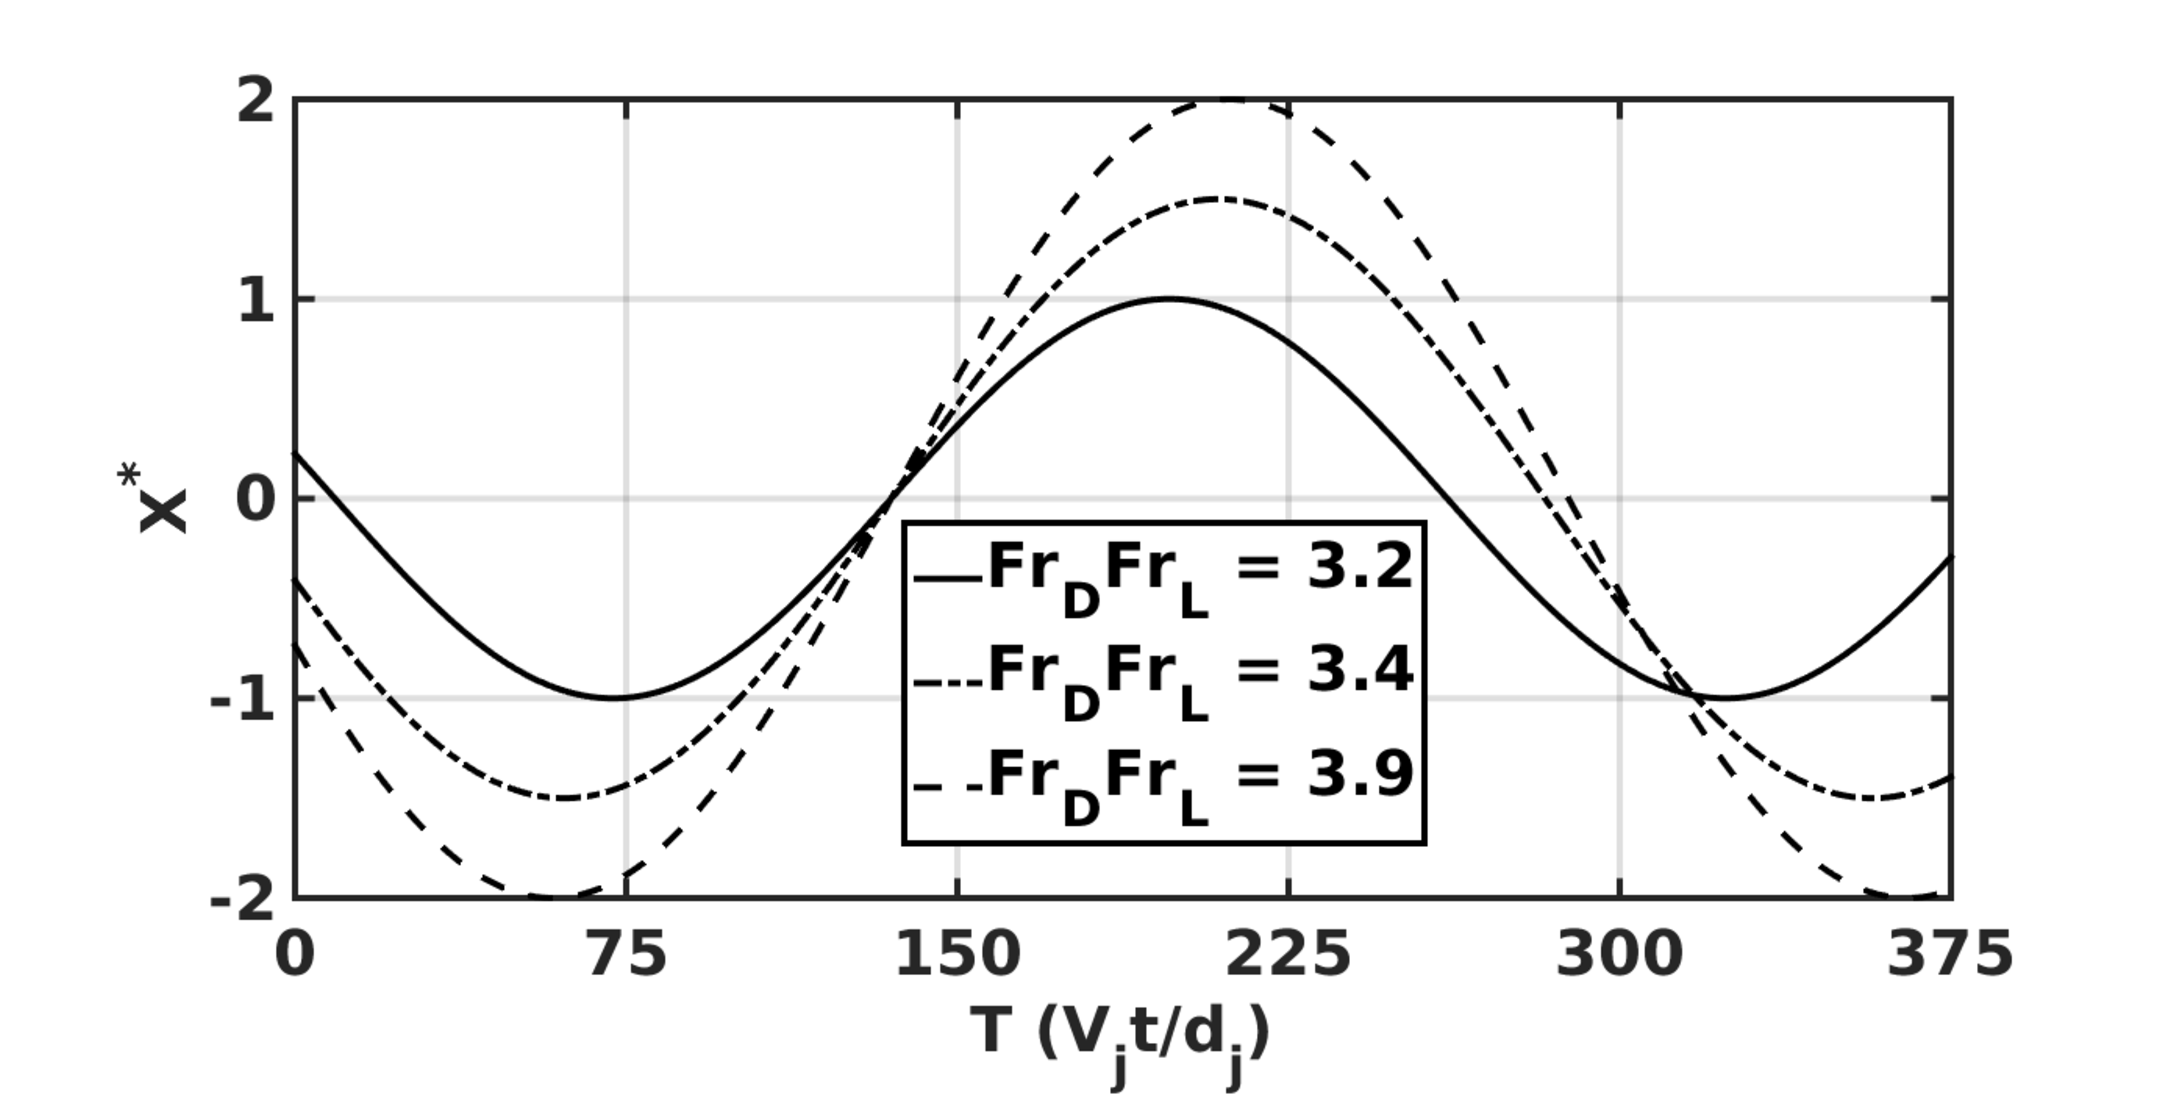
\includegraphics[width=\linewidth]{chapters/jetPool/Figure17}
	\caption{Temporal variation of the normalized abscissa of the centroid related to the entrainment cluster.}
	\label{figure::solution}
\end{figure}
\subsection{Kinematics of the cluster centroid}
From a close look at experimental snaps, it has been observed that the centroid of the projected area (location x) shows periodic oscillation. Binary two-dimensional images, as shown in Figure~\ref{Fig::setup} (b), are used to calculate the location of the centroid. Equation~\ref{Equation::xintegration} is followed for calculation, where $\bar{x}$($x_i , y_i$) is the location of the pixel in the binary image corresponding to the cluster area (non-zero value) and N is the total number of non-zero pixels.
\begin{equation}
X_{centroid} = \frac{\int \bar{x}dA}{A} = \frac{\sum_{i = 1}^{N}\bar{x_i}}{N}
\label{Equation::xintegration}
\end{equation}
\begin{figure}
	\centering
	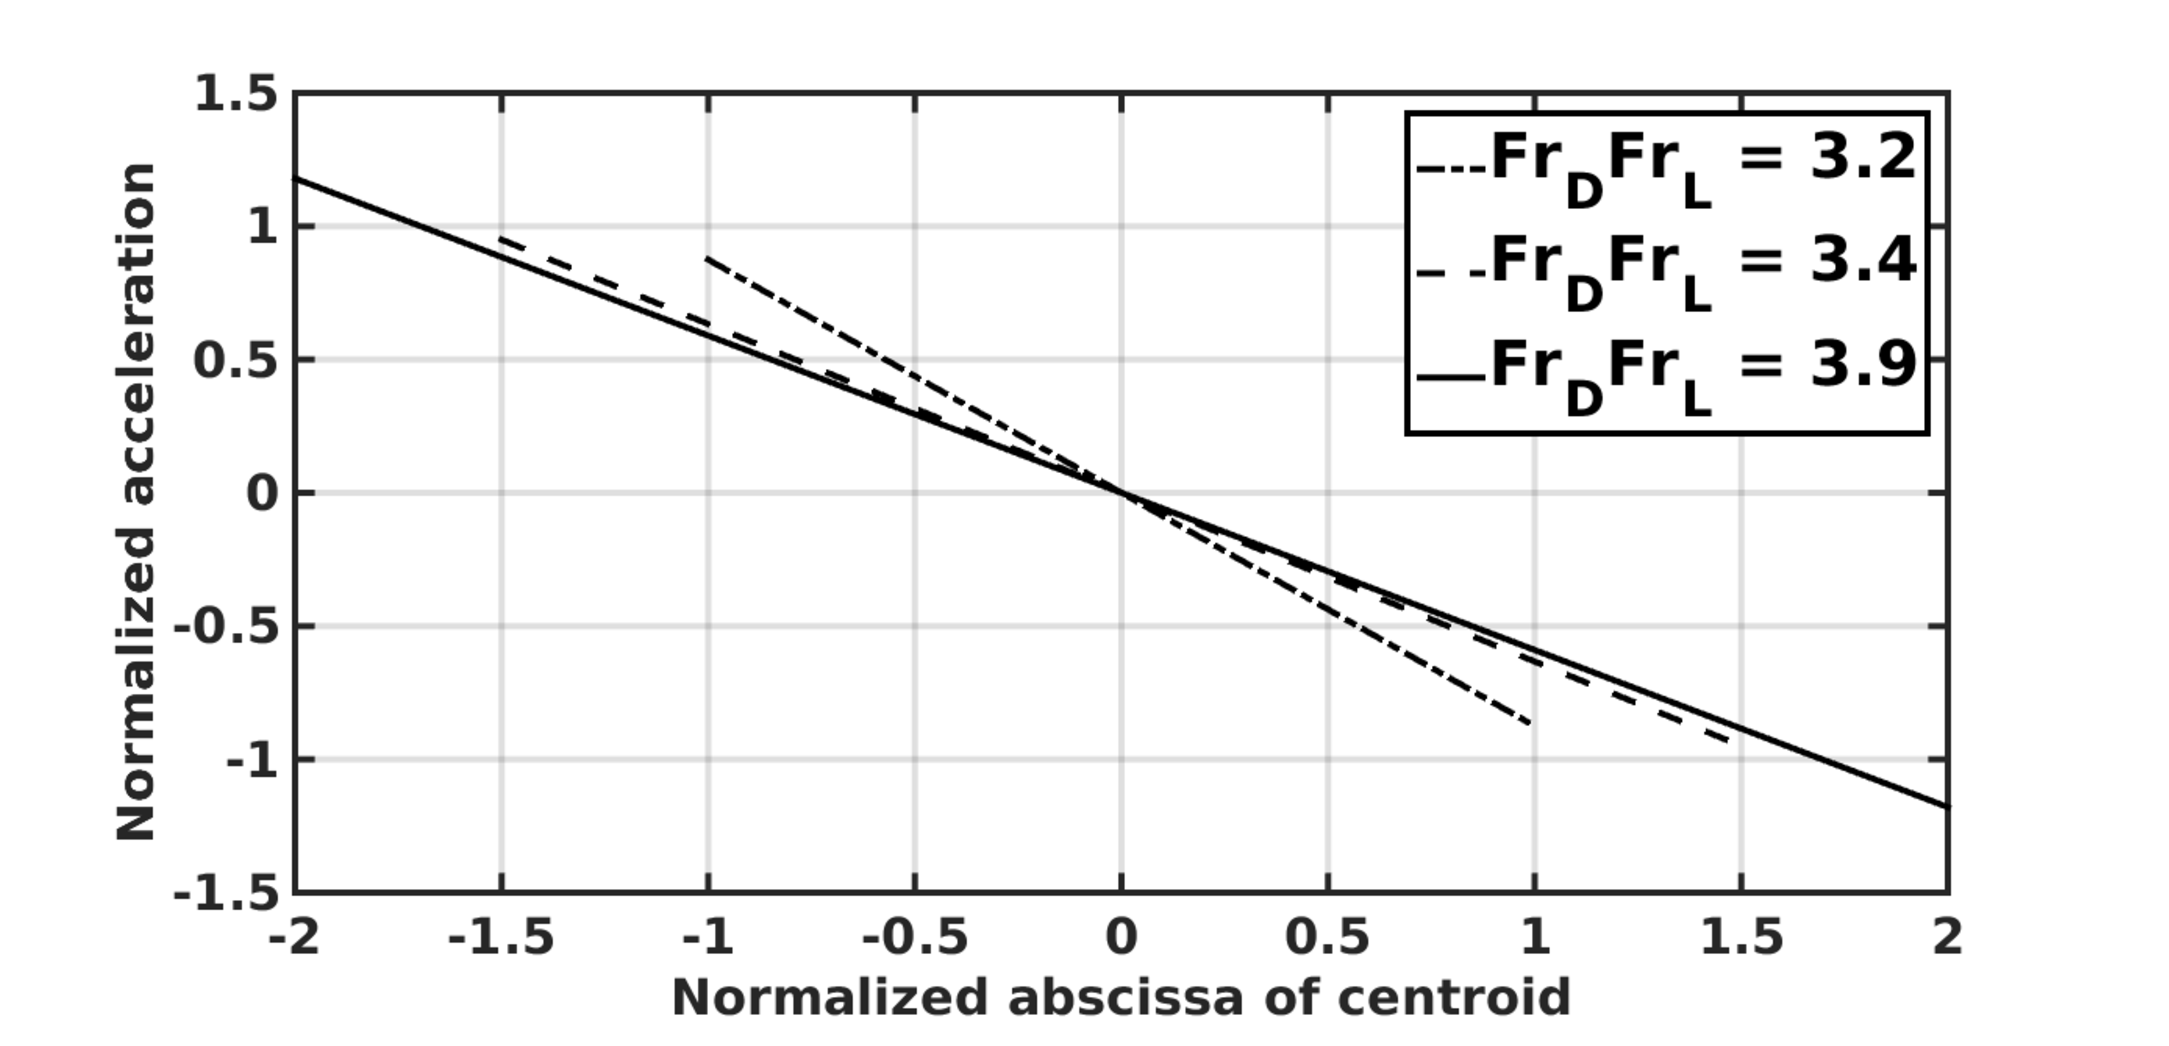
\includegraphics[width=\linewidth]{chapters/jetPool/Figure18}
	\caption{Variation of the acceleration of the centroid with its normalized abscissa related to the entrainment cluster.}
	\label{figure::acc}
\end{figure}
Upon non-dimensionalizing with its mean and standard deviation as $ X^{*} = \left(\frac{x-mean(x)}{\sigma_{x}}\right)$, the periodic movement as illustrated in equation~\ref{Equation::eqShm} is obtained.
\begin{equation}
\frac{\partial^2 X^*}{\partial t^2} + \omega^2X^{*} = 0
\label{Equation::eqShm}
\end{equation} 
Oscillations are observed in phases at all azimuthal planes. This represents the pseudo-randomness of the bubble cluster configuration having constant depth over time. As cluster is constructed by pinch off of bubbles from free surface, temporal dependence is not eliminated and became prompt in the lateral direction. From experimental observation, variation of $X^*$ is obtained with non-dimensional time ($T = V_jt/d_j$) and plotted in Figure~\ref{figure::solution}.
The periodic nature is clearly depicted in Figure~\ref{figure::solution} having higher amplitude for lower $Fr_DFr_L$. Increase of $\omega$ for lower $Fr_DFr_L$ can also be seen from this figure as oscillation time periods for $Fr_DFr_L$ = 3.2 is lower than $Fr_DFr_L$ = 3.9. In equation~\ref{Equation::eqShm}, acceleration of centroid for the bubble cluster varies proportionally with its shift from the longitudinal jet plane. To depict that clearly, in Figure~\ref{figure::acc}, normalized acceleration for different experimental conditions of $Fr_DFr_L$ is shown. In all these cases, linear patterns have been observed confirming the validity of equation~\ref{Equation::eqShm}. At higher $Fr_DFr_L$, it has been observed that the centroid acceleration increases and it deviates more from the jet plane. Acceleration of the centroid increases at a faster rate with shift from jet plane for lower $Fr_DFr_L$ (resulting in higher proportionality constant $ \omega^2 $ in equation~\ref{Equation::eqShm}). \\
Present experimental effort establishes the steady overall behavior of the cluster but keeps provision for monitoring the local behavior of bubbles. Next section targets towards an understanding of individual bubble dynamics with the help of visualization and signals from electrical conductivity probe.
\section{Bubble kinematics}
\begin{figure}
	\centering'
	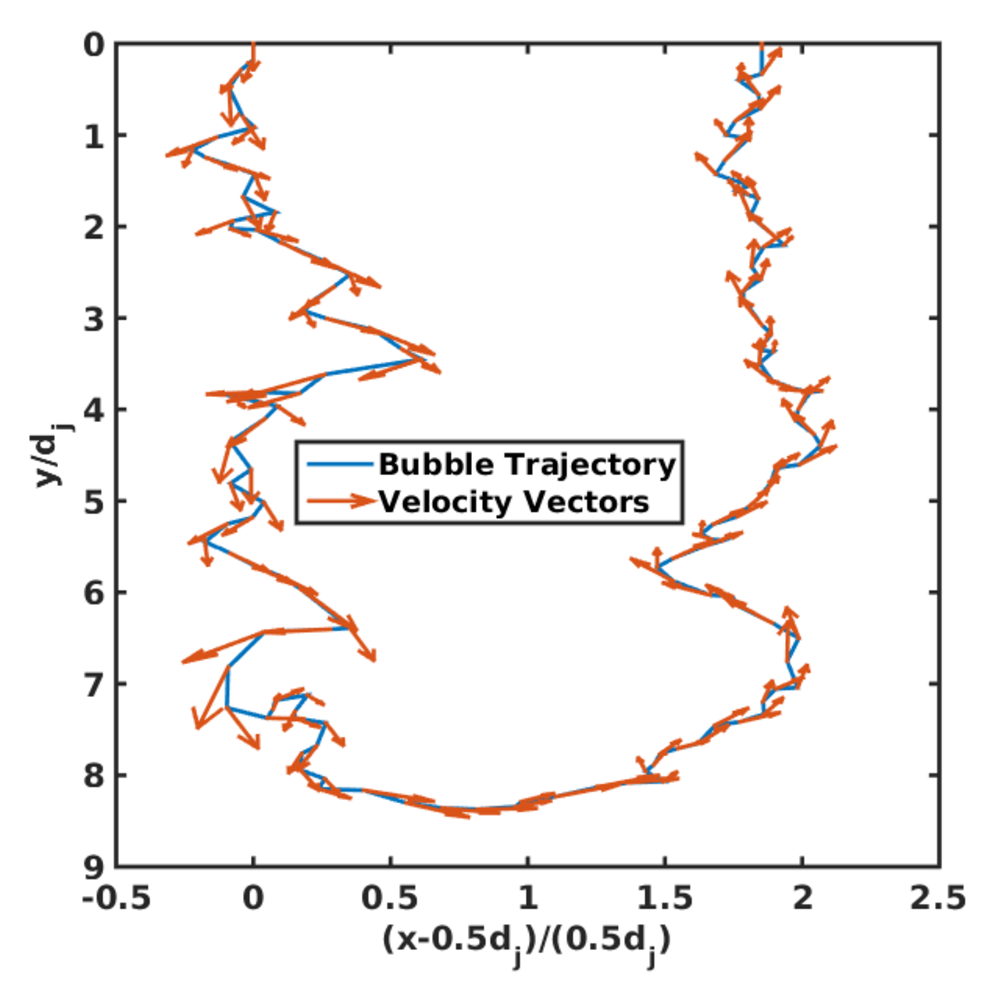
\includegraphics[width=0.5\linewidth]{chapters/jetPool/Figure19}
	\caption{Bubble trajectory in the entrained region at $Fr_DFr_L = 1.8$, as obtained from experimental observation. The bubble inception occurs at the tip of the thin air sheathe, traverses through the entrainment region, stops the downward motion as the buoyancy dominates its motion and erupts back at the free surface.}
	\label{Figure::bubble}
\end{figure}
The bubble cluster consists different sized bubbles consistently making and breaking within the triangular entrainment region. The trajectory of a bubble is followed at a comparatively low-speed entrainment phenomenon from photographic observation in experiments and represented in Figure~\ref{Figure::bubble}. After birth, the bubble moves downwards inside the cluster and reaches the maximum depth. It halts there for sometime before coming up from the other side of the cluster. Its downward movement is driven by inertia and upward movement is due to buoyancy pull. Instantaneous velocity in the plot is also shown. In between initiation and collapse, the bubble is dominated by inertia, interaction and buoyancy pull inside the cluster (Figure~\ref{Figure::bubble}). \\
\begin{figure}
	\centering
	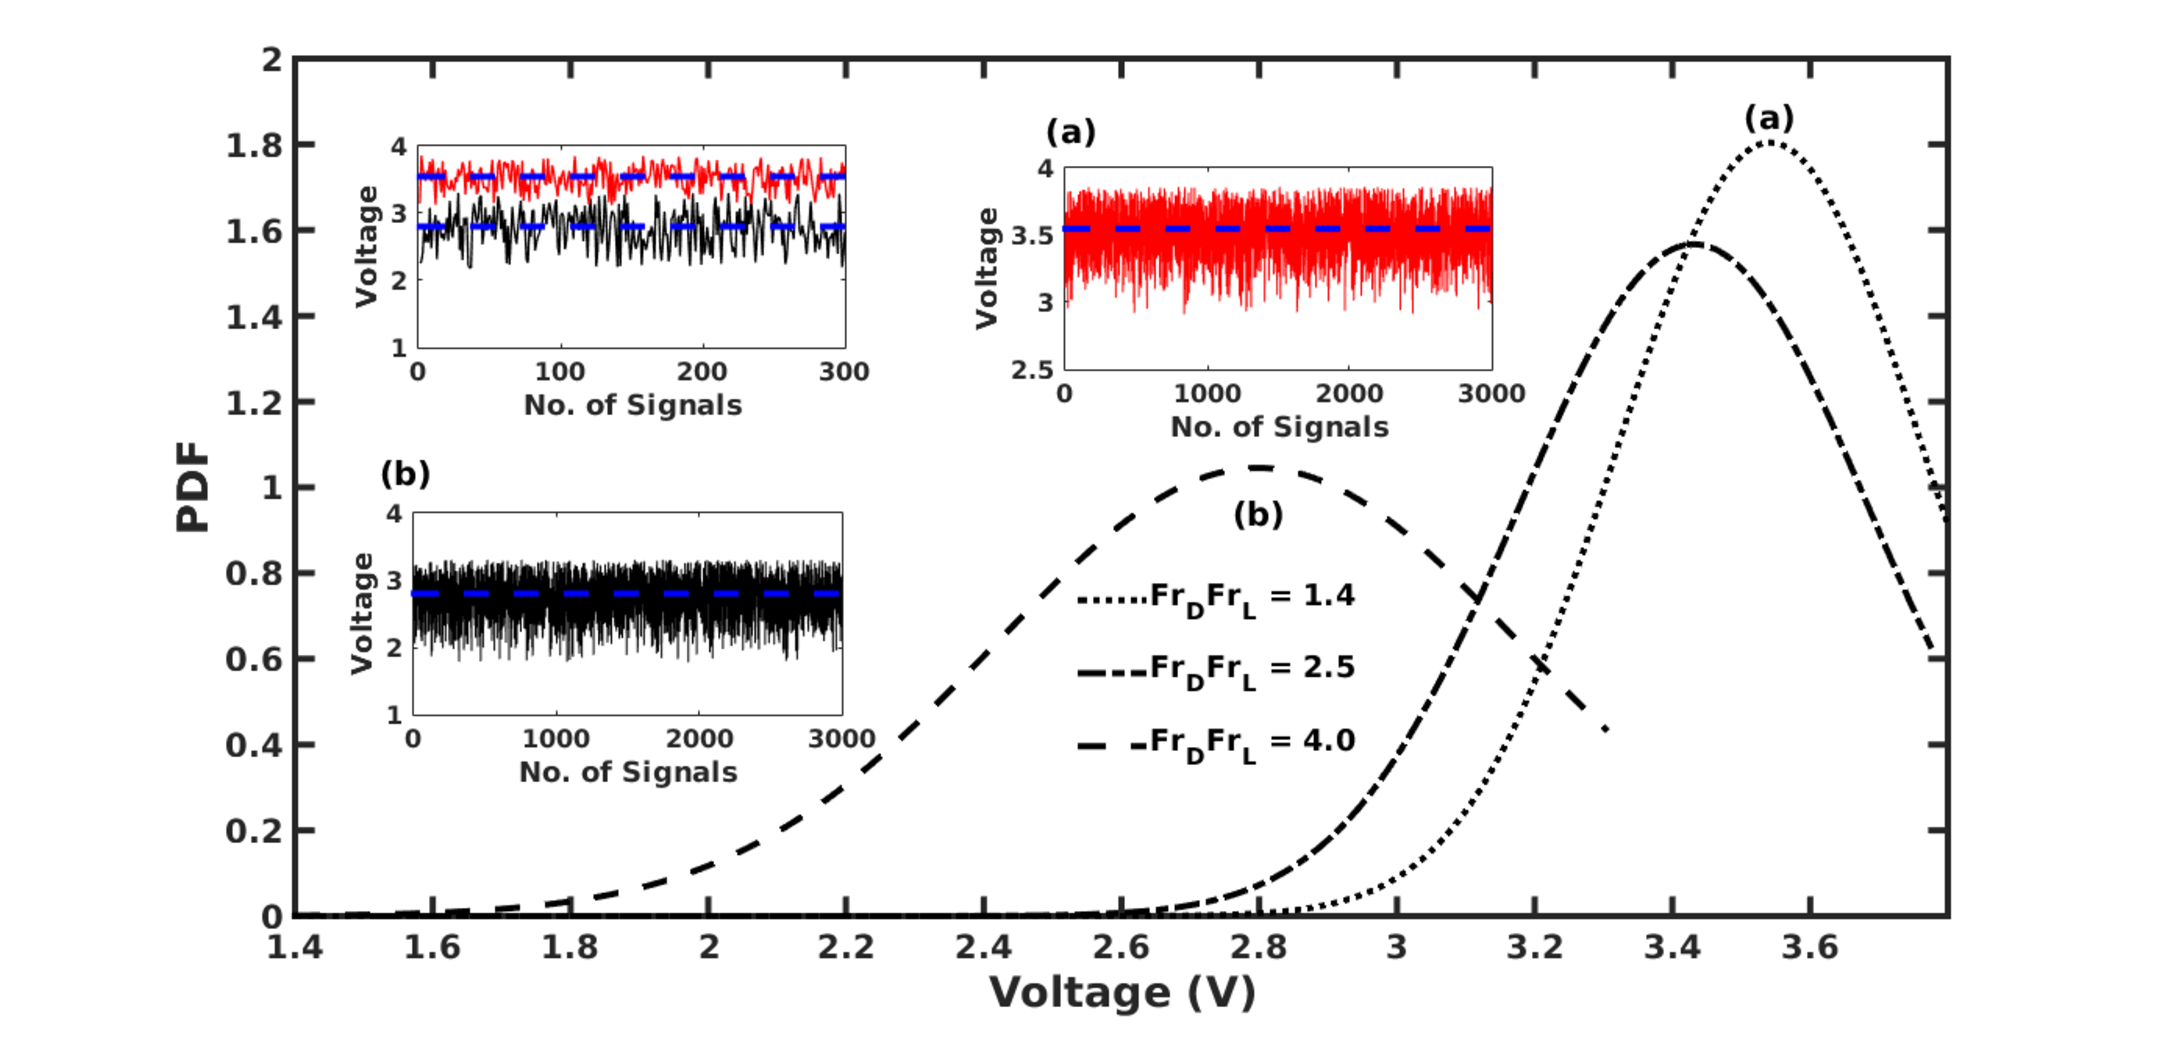
\includegraphics[width=\linewidth]{chapters/jetPool/Figure20}
	\caption{Characteristic probability density function of the experimental probe signals at different values of $Fr_DFr_L$. More the peak is shifted towards the left, the high density of bubbles are present at the spatial location of the electrodes.}
	\label{Figure::pdf}
\end{figure}
Electrical conductivity probe signals have been recorded for varying flow rates and different lengths of jets inside the bubble entrainment zone. The physical illustration of the voltage signal is shown in Figure~\ref{Figure::show}. The sharp downfalls represent the presence of bubbles. A representative signal of probes in the experimental cluster is shown in the inset of Figure~\ref{Figure::pdf}. Even though the voltage signal, which varies in between 3.5 to 1.5 volts, clearly depicts the presence of entrapped air bubbles, it is difficult to get any kinematic inference. Therefore, from raw electrical signals, probability density function (PDF) has been plotted for three representative flow-rates in Figure~\ref{Figure::pdf}. The peak in PDF shifts to the left and lowers down as the flow rate increases. The probability of getting lower voltage signifies vigorous cluster characteristics and high probability of bubble presence at a given spatial coordinate. With an increase in jet flow-rate, entrainment strength increases and causes peak at the lower voltage. This shows more and more bubbles are being trapped due to its random presence in the cluster at higher flow rates. This clearly demonstrates the bubble kinematics as well as cluster vibrations. Signals of probe confirm the presence of a bubble in the cluster and its peak of PDF at lower value signifies higher mobility of bubbles at the cluster. At lower jet speed bubbles are produced but exhibit comparative calm behavior to have a liquid contact at the probe tip. On the other hand, at high jet speed, random motion of the generated bubble keeps always gaseous phase in contact with the probe. Present observation establishes highly random kinematic behavior at high jet speed.
\section{Summary}
Impingement of water jet on a pool is studied using full-scale experiments and detailed numerical simulation. High-speed imaging and electrical conductivity probes are used in experimental instrumentation. Depending on jet's strength, two opposite regimes have been identified as no entrainment and conical bubble cluster. Formation of inertia dominated cavity and surface tension dominated collapse have been identified as the basic consequences of the onset of bubble entrainment as a cluster. Repetitive formation and breakage of air cavity in the pool results in disconnected but interacting bubble population. The mutual interplay between inertia and surface tension determines the depth of entrained region which has been reported as a function of the product of Froude Numbers  ($Fr_DFr_L$) in two correlations for different regimes with the boundary at $Fr_DFr_L = 1.2$. Proposed correlation shows accurate prediction (R-squared of $0.9$ and $0.95$) of depth for a wide range of jet diameters and heights. Using high-speed images, increasing projected area of entrainment has been observed for higher $Fr_DFr_L$ and time which establishes the affected zone during entrainment. Kinematics of entrainment has been studied using a spatio-temporal variation of centroid location of the cluster. Acceleration of the centroid is found to be linearly varying with the deviation of the entrained region from the plane of jet impact. The trajectory of a single bubble has been also reported in the study from visualization to establish formation, downward traverse, stabilized floating at critical height, buoyancy-driven approach towards free surface and collapse in its whole life cycle.
